\PassOptionsToPackage{brazilian}{babel}
\documentclass[
	12pt,
	a4paper,
	article,
	twocolumn
]{abntex2}

% --- Pacotes Básicos e Hifenação em Português ---
\usepackage[brazilian]{babel}
\usepackage[utf8]{inputenc}
\usepackage[T1]{fontenc}
\usepackage{lmodern}
\usepackage{indentfirst}
\usepackage{graphicx}
\graphicspath{{figuras/}{./}}
\usepackage{amsmath,amssymb}
\usepackage{booktabs}
\usepackage{enumitem}
\usepackage{hyperref}

\hypersetup{
	colorlinks=true,
	linkcolor=blue,
	citecolor=blue,
	urlcolor=blue
}

% Remove o título em língua estrangeira padrão do abntex2 article
\renewcommand{\maketitlehookb}{}

\titulo{Mini-projeto 2: visão computacional com redes neurais (MLP vs.\ CNN no MNIST)}

\autor{
	Eduardo N. S. R.\\[0.2em]
	\small PPGCO / PGC112 -- Faculdade de Computação (FACOM)\\
	\small Repositório Github: \href{https://github.com/vndmtrx/ppgco-pgc112-ia}{\texttt{vndmtrx/ppgco-pgc112-ia}}
}

\data{Uberlândia -- MG, Brasil, 2026}

\begin{document}
\frenchspacing
\SingleSpacing

\maketitle

\section{Introdução}

Este relatório analisa duas famílias de redes neurais implementadas em PyTorch~\cite{paszke2019} para classificar os dígitos do \textbf{MNIST}~\cite{russell2020,smola2023}: um Perceptron Multicamadas (MLP) com saída Softmax e uma Rede Neural Convolucional (CNN) no estilo LeNet. O foco não é só a acurácia final, mas entender o preço de destruir a geometria da imagem ao achatá-la, quanto custa cada arquitetura em parâmetros e CPU, e que tipos de dígitos continuam confundindo os modelos.

Todo o código, os testes automatizados e os registros brutos estão em \texttt{mini\_projeto\_2} no repositório \url{https://github.com/vndmtrx/ppgco-pgc112-ia}, com o passo a passo de execução no \texttt{README.md}.

\section{Dados e Métricas de Avaliação}

O MNIST (carregado via \texttt{torchvision.datasets.MNIST}) reúne $70.000$ imagens em tons de cinza ($28 \times 28$ pixels) divididas entre $60.000$ de treino e $10.000$ de teste oficial. Para calibrar hiperparâmetros sem viciar a seleção no teste, separou-se o treino original de forma determinística (\texttt{seed=42}, em \texttt{dataset.py}) em \textbf{$50.000$ imagens de treino} e \textbf{$10.000$ de validação}. O conjunto de teste permaneceu lacrado até a escolha final de cada modelo.

\noindent\textbf{Normalização Empírica.} Medindo os pixels em $[0, 1]$ diretamente no subconjunto de treino, foram obtidas média $\mu = 0{,}1307$ e desvio padrão $\sigma = 0{,}3081$. Essa média baixa reflete a esparsidade dos traços: cerca de $87\%$ do quadro é fundo preto. Aplicou-se a padronização $z = (x - \mu)/\sigma$ para centralizar as entradas na origem e evitar gradientes enviesados por escala.

\medskip
\noindent\textbf{Balanceamento e Métricas.} Os três subconjuntos mantêm distribuição equilibrada entre os dígitos (Figura~\ref{fig:dist_classes}). No treino, a contagem vai de $4.546$ (dígito $5$) a $5.613$ ($1$); na validação, de $875$ ($5$) a $1.129$ ($1$, ou $11{,}29\%$); e no teste, de $892$ ($5$) a $1.135$ ($1$). A Figura~\ref{fig:exemplos_digitos} mostra amostras típicas das dez classes. Todas as execuções foram avaliadas por acurácia global, precisão, revocação, F1-score macro e matriz de confusão $10 \times 10$.

\begin{figure}[htbp]
\centering
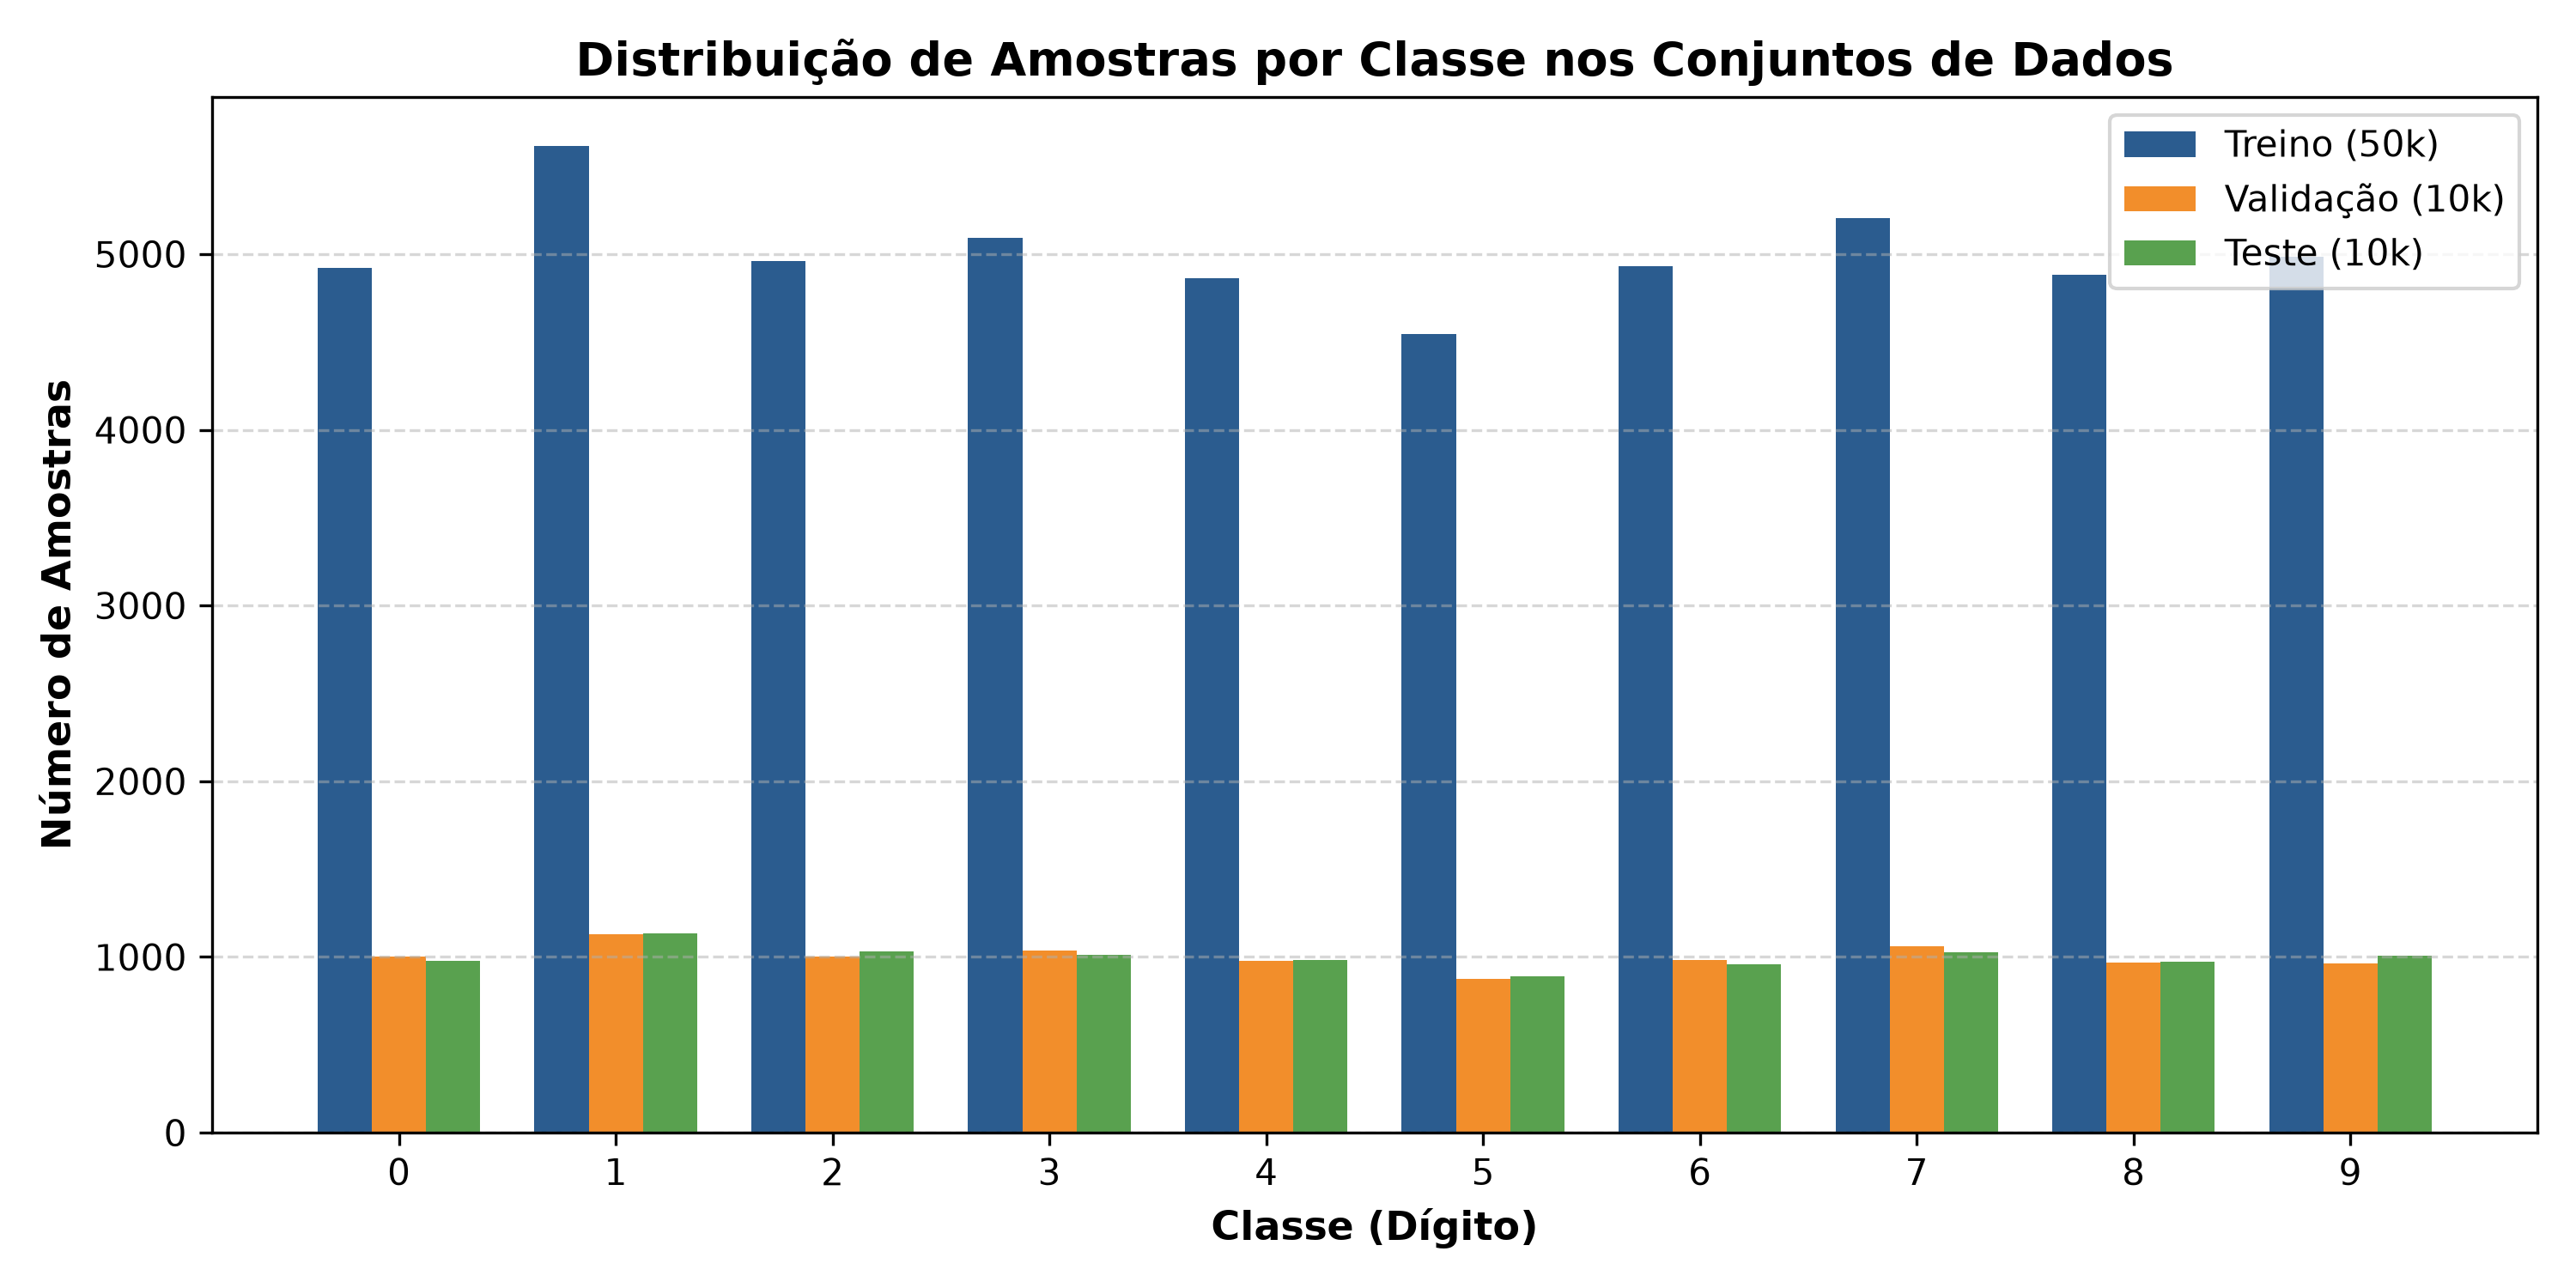
\includegraphics[width=0.78\columnwidth]{distribuicao_classes.png}
\caption{Distribuição por classe nos conjuntos de treino ($50\text{k}$), validação ($10\text{k}$) e teste ($10\text{k}$).}
\label{fig:dist_classes}
\end{figure}

\begin{figure}[htbp]
\centering
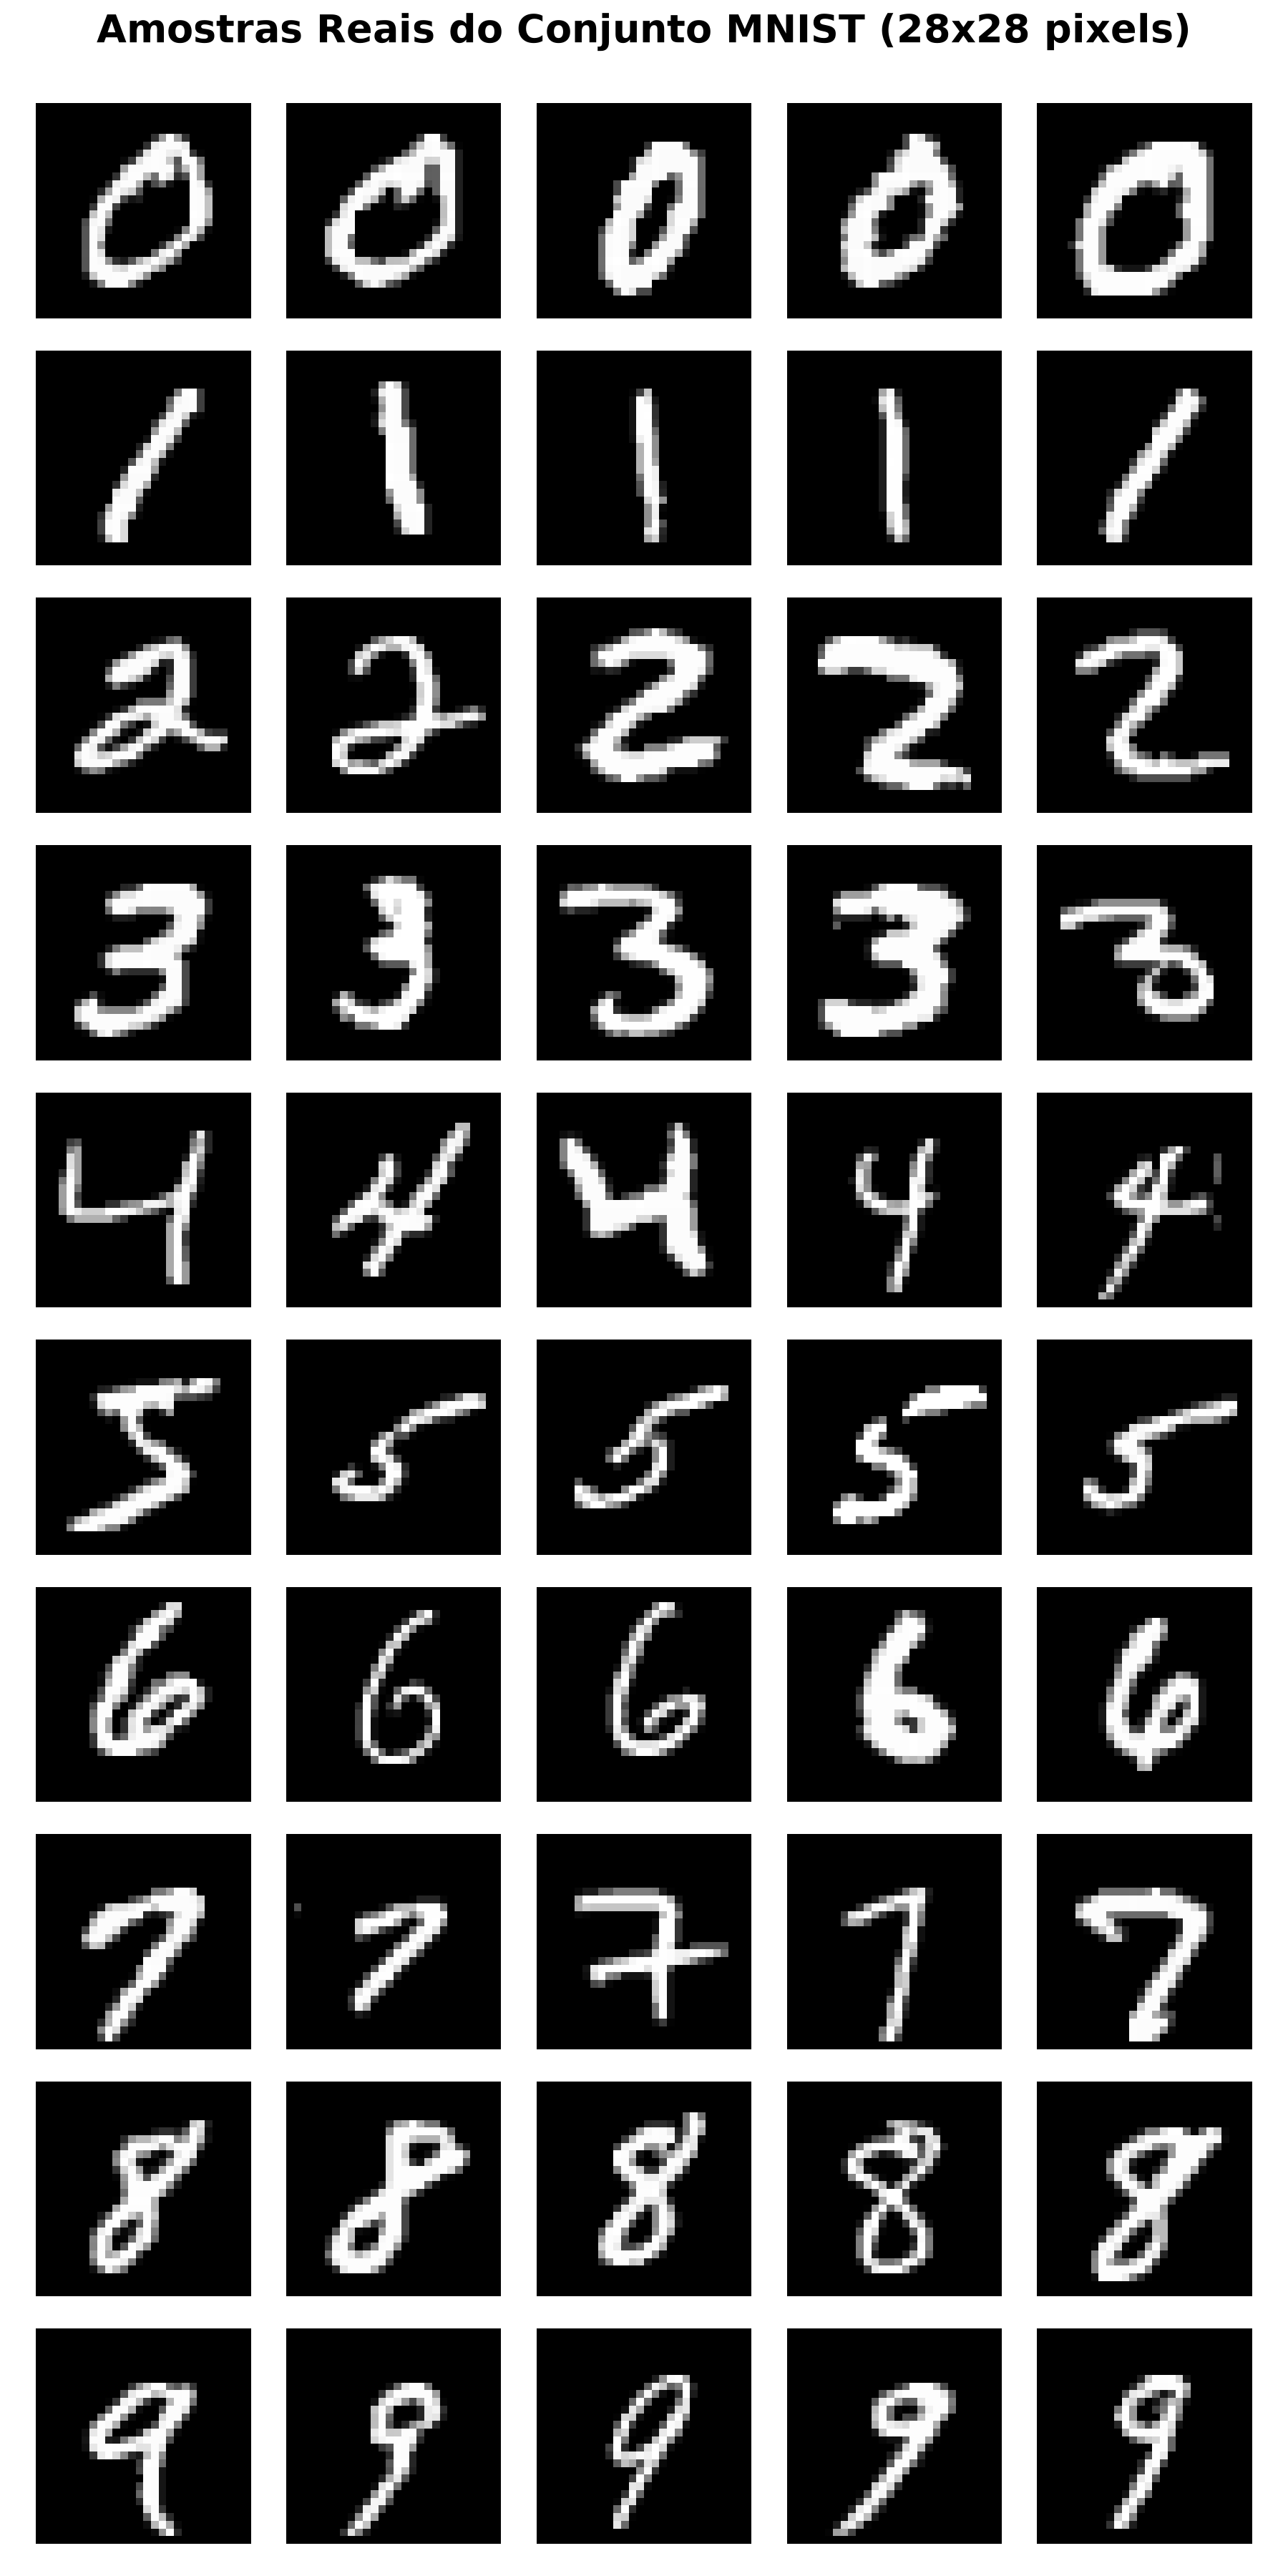
\includegraphics[width=0.34\columnwidth]{exemplos_digitos.png}
\caption{Exemplos de dígitos ($28 \times 28$) do MNIST.}
\label{fig:exemplos_digitos}
\end{figure}

\section{MLP com Softmax}

\subsection{Sobre o Método e Cegueira Espacial}

O MLP é uma rede de alimentação direta (\textit{feed-forward}), sem conexões recorrentes, composta por camada de entrada, camadas lineares ocultas com ativação não linear ReLU e camada de saída Softmax~\cite{smola2023}. A rede recebe um vetor unidimensional $\mathbf{x} \in \mathbb{R}^{784}$ gerado pelo achatamento $28 \times 28 \to 784$. Cada camada linear oculta calcula $\mathbf{h}^{(l)} = \max(\mathbf{0}, \mathbf{W}^{(l)} \mathbf{h}^{(l-1)} + \mathbf{b}^{(l)})$, até projetar em $10$ \textit{logits} $\mathbf{z} \in \mathbb{R}^{10}$. Na saída, a função Softmax converte esses \textit{logits} em probabilidades $P(y = k \mid \mathbf{x}) = e^{z_k} / \sum_{j=0}^{9} e^{z_j}$, otimizadas pela entropia cruzada $\mathcal{L} = -\ln P(y = y_{\text{real}} \mid \mathbf{x})$ (via \texttt{nn.CrossEntropyLoss}, que junta \texttt{LogSoftmax} e \texttt{NLLLoss} sem risco de \textit{overflow}).

\medskip
\noindent\textbf{Por que o MLP ignora a estrutura espacial.} Achatar uma grade $28 \times 28$ equivale a fatiar a imagem em $28$ linhas horizontais e colá-las em sequência. Pixels vizinhos na mesma linha permanecem adjacentes (exceto nas bordas entre linhas), mas vizinhos verticais ficam separados por exatamente $28$ posições e as diagonais se rompem. Como $\mathbf{W}^{(1)}\mathbf{x}$ multiplica cada entrada por uma coluna própria, qualquer permutação fixa aplicada a todos os pixels gera o mesmo problema para a rede, bastando reordenar as colunas de $\mathbf{W}^{(1)}$. O MLP entra sem nenhum viés geométrico e precisa gastar parâmetros para redescobrir do zero relações entre traços próximos.

\subsection{Implementação e Seleção Pela Validação}

O MLP configurável com ReLU (\texttt{models/mlp.py}) e SGD puro foi implementado mantendo o conjunto de teste isolado durante toda a busca. Para comparar hiperparâmetros de forma limpa, conduziu-se a bateria \texttt{v5} em CPU (\texttt{executar\_bateria\_v5.sh}): $15$ configurações em blocos \textit{ceteris paribus} cobrindo largura ($64$ a $1024$), profundidade ($1$ a $3$ camadas), lote ($64$ a $512$), taxa $\eta \in \{0{,}05, 0{,}1, 0{,}2\}$ e momento ($0$ ou $0{,}9$), repetidas com $3$ sementes por até $50$ épocas ($45$ treinos). Em cada execução, foi salvo o \textit{checkpoint} de menor perda de validação.

A Tabela~\ref{tab:mlp_val} traz os recortes principais. A acurácia de validação sobe até $512$ neurônios ($97{,}95 \pm 0{,}08\%$) e estaciona em $1024$ ($97{,}93 \pm 0{,}12\%$). Como o erro-padrão em $N = 10.000$ é cerca de $0{,}14\text{ p.p.}$, dobrar os pesos não traz ganho estatístico real. Nos demais blocos, o lote $64$ com momento $0{,}9$ foi o mais instável ($94{,}50 \pm 1{,}12\%$) por somar gradientes ruidosos a passos amplos, enquanto zerar o momento ($m = 0$) atrasou o ponto ótimo das épocas $5$--$10$ para as épocas $32$--$36$. Selecionou-se a arquitetura de \textbf{1 camada oculta com $512$ neurônios} ($784 \to 512 \to 10$, $407.050$ parâmetros, lote $256$, $\eta = 0{,}1$, momento $0{,}9$).

Essa escolha corrigiu também uma leitura apressada sobre profundidade. Olhando apenas o critério pré-definido de menor perda, redes de $2$ e $3$ camadas parecem inferiores à camada única. Contudo, em $44$ das $45$ execuções, a época $50$ atingiu acurácia de validação maior que o \textit{checkpoint} de perda mínima ($+0{,}47\text{ p.p.}$ em média), ao preço de elevar a perda média em $1{,}47\times$ pelo excesso de confiança nos erros residuais. Pela acurácia da época $50$, a rede $512 \to 256$ passaria à frente ($98{,}28\%$ contra $97{,}99\%$ da camada única). Mantiveram-se os pesos da menor perda porque o critério foi travado antes da bateria.

\begin{table}[htbp]
\centering
\caption{Seleção do MLP na validação ($3$ sementes, $50$ épocas).}
\label{tab:mlp_val}
\resizebox{\columnwidth}{!}{%
\begin{tabular}{lrrrrr}
\toprule
Configuração & Parâm. & Acc Val (\%) & Perda Val & Ép. & Tempo (s) \\
\midrule
$h=[64]$, $b=256, \eta=0{,}1, m=0{,}9$ & $50.890$ & $96{,}82 \pm 0{,}23$ & $0{,}1139$ & $4{,}3$ & $29$ \\
$h=[300]$, $b=256, \eta=0{,}1, m=0{,}9$ & $238.510$ & $97{,}78 \pm 0{,}16$ & $0{,}0806$ & $7{,}3$ & $53$ \\
\textbf{$h=[512]$, $b=256, \eta=0{,}1, m=0{,}9$} & $\mathbf{407.050}$ & $\mathbf{97{,}95 \pm 0{,}08}$ & $0{,}0744$ & $8{,}3$ & $54$ \\
$h=[1024]$, $b=256, \eta=0{,}1, m=0{,}9$ & $814.090$ & $97{,}93 \pm 0{,}12$ & $0{,}0708$ & $7{,}0$ & $85$ \\
$h=[300, 100]$, $b=256, \eta=0{,}1, m=0{,}9$ & $266.610$ & $97{,}64 \pm 0{,}22$ & $0{,}0930$ & $6{,}3$ & $51$ \\
$h=[512, 256]$, $b=256, \eta=0{,}1, m=0{,}9$ & $535.818$ & $97{,}60 \pm 0{,}16$ & $0{,}0818$ & $3{,}7$ & $74$ \\
$h=[300]$, $b=64, \eta=0{,}1, m=0{,}9$ & $238.510$ & $94{,}50 \pm 1{,}12$ & $0{,}2456$ & $3{,}3$ & $75$ \\
$h=[300]$, $b=256, \eta=0{,}1, m=0{,}0$ & $238.510$ & $97{,}62 \pm 0{,}01$ & $0{,}0769$ & $33{,}7$ & $43$ \\
\bottomrule
\end{tabular}%
}
\end{table}

\subsection{Experimento e Análise de Erros do MLP}

Na Figura~\ref{fig:mlp_perda}, o treino da semente escolhida ($53{,}03\text{ s}$ no total) atinge a menor perda de validação na \textbf{época 7} ($0{,}0720$, com $97{,}99\%$ de acurácia). Depois disso o modelo passa a aumentar a confiança nos erros residuais e a validação piora. Ao abrir o teste oficial uma única vez (\texttt{mlp\_v5\_testar.py}), o MLP obteve \textbf{$98{,}19\%$ de acurácia} ($181$ erros em $10.000$), perda de $0{,}06039$, precisão macro de $98{,}19\%$, revocação macro de $98{,}17\%$ e \textbf{F1 macro de $98{,}18\%$} (Figura~\ref{fig:mlp_cm}). Por classe, o dígito $1$ alcançou a maior revocação ($99{,}56\%$, traço único e estável), e o $9$ teve o pior desempenho ($97{,}22\%$).

\begin{figure}[htbp]
\centering
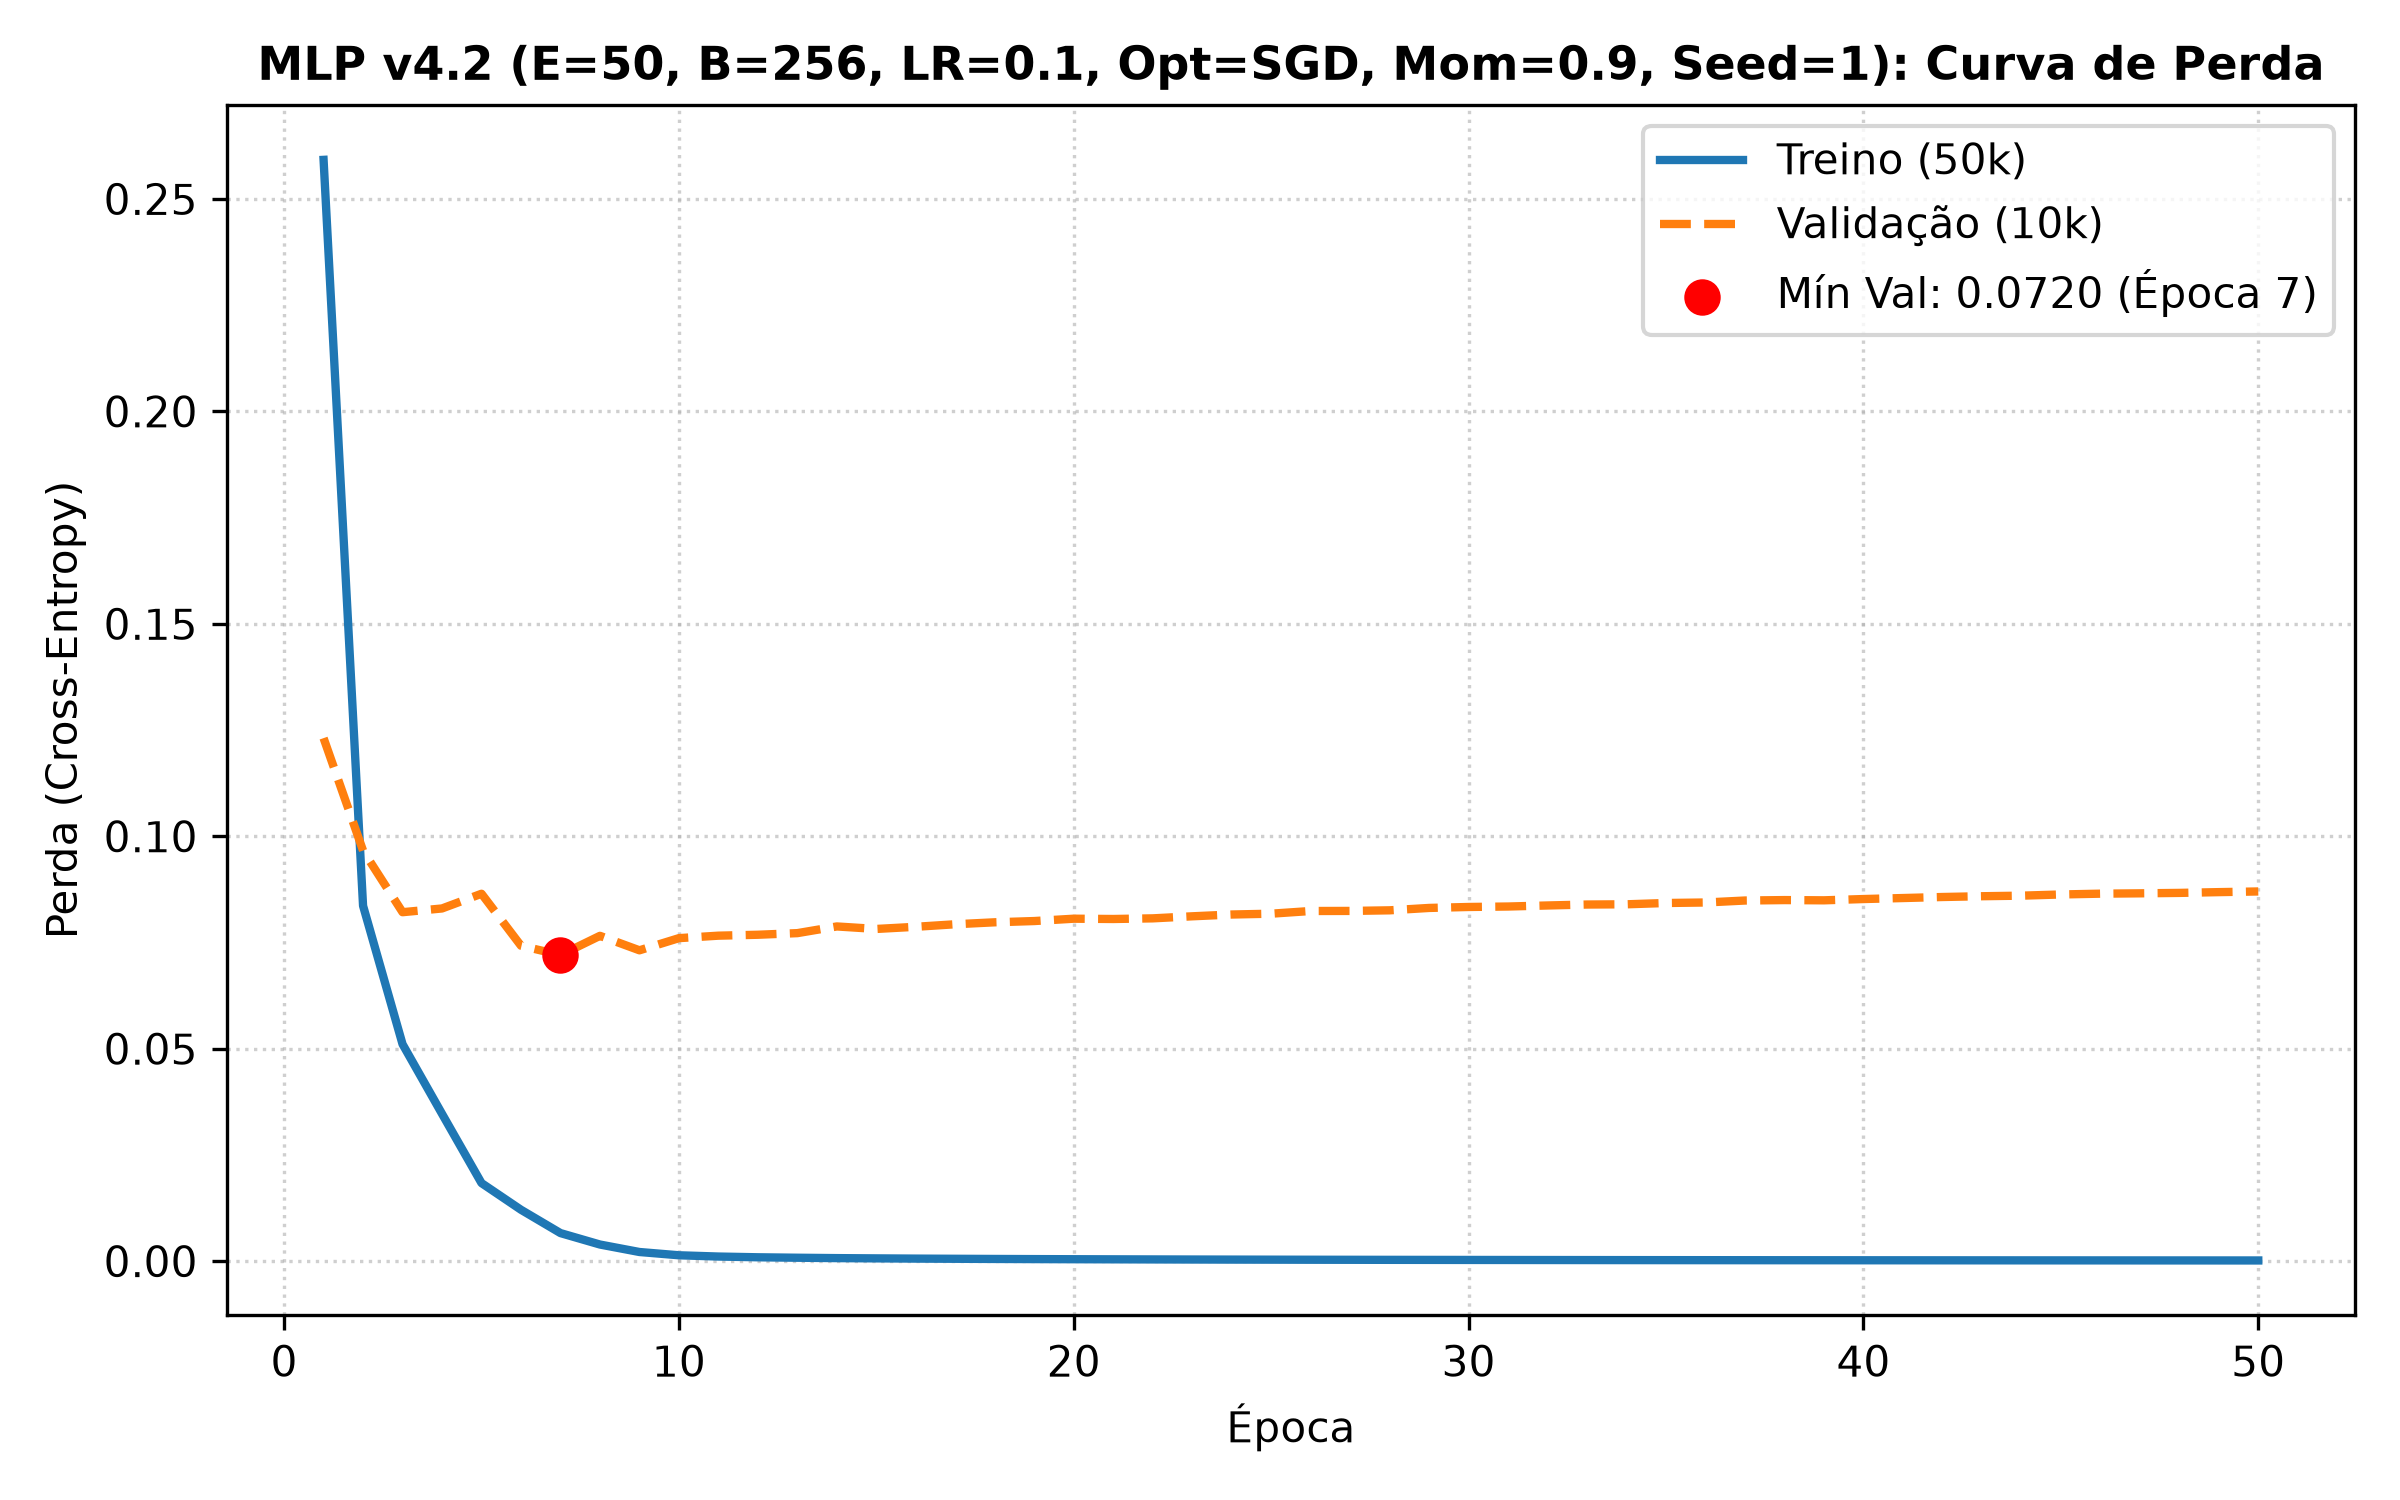
\includegraphics[width=0.74\columnwidth]{v5_e50_b256_lr0.1_m0.9_h512_s1/mlp_treinado_v5_e50_b256_lr0.1_m0.9_h512_s1_perda.png}
\caption{Curva de perda do MLP campeão ($784 \to 512 \to 10$, mínimo na época $7$).}
\label{fig:mlp_perda}
\end{figure}

\begin{figure}[htbp]
\centering
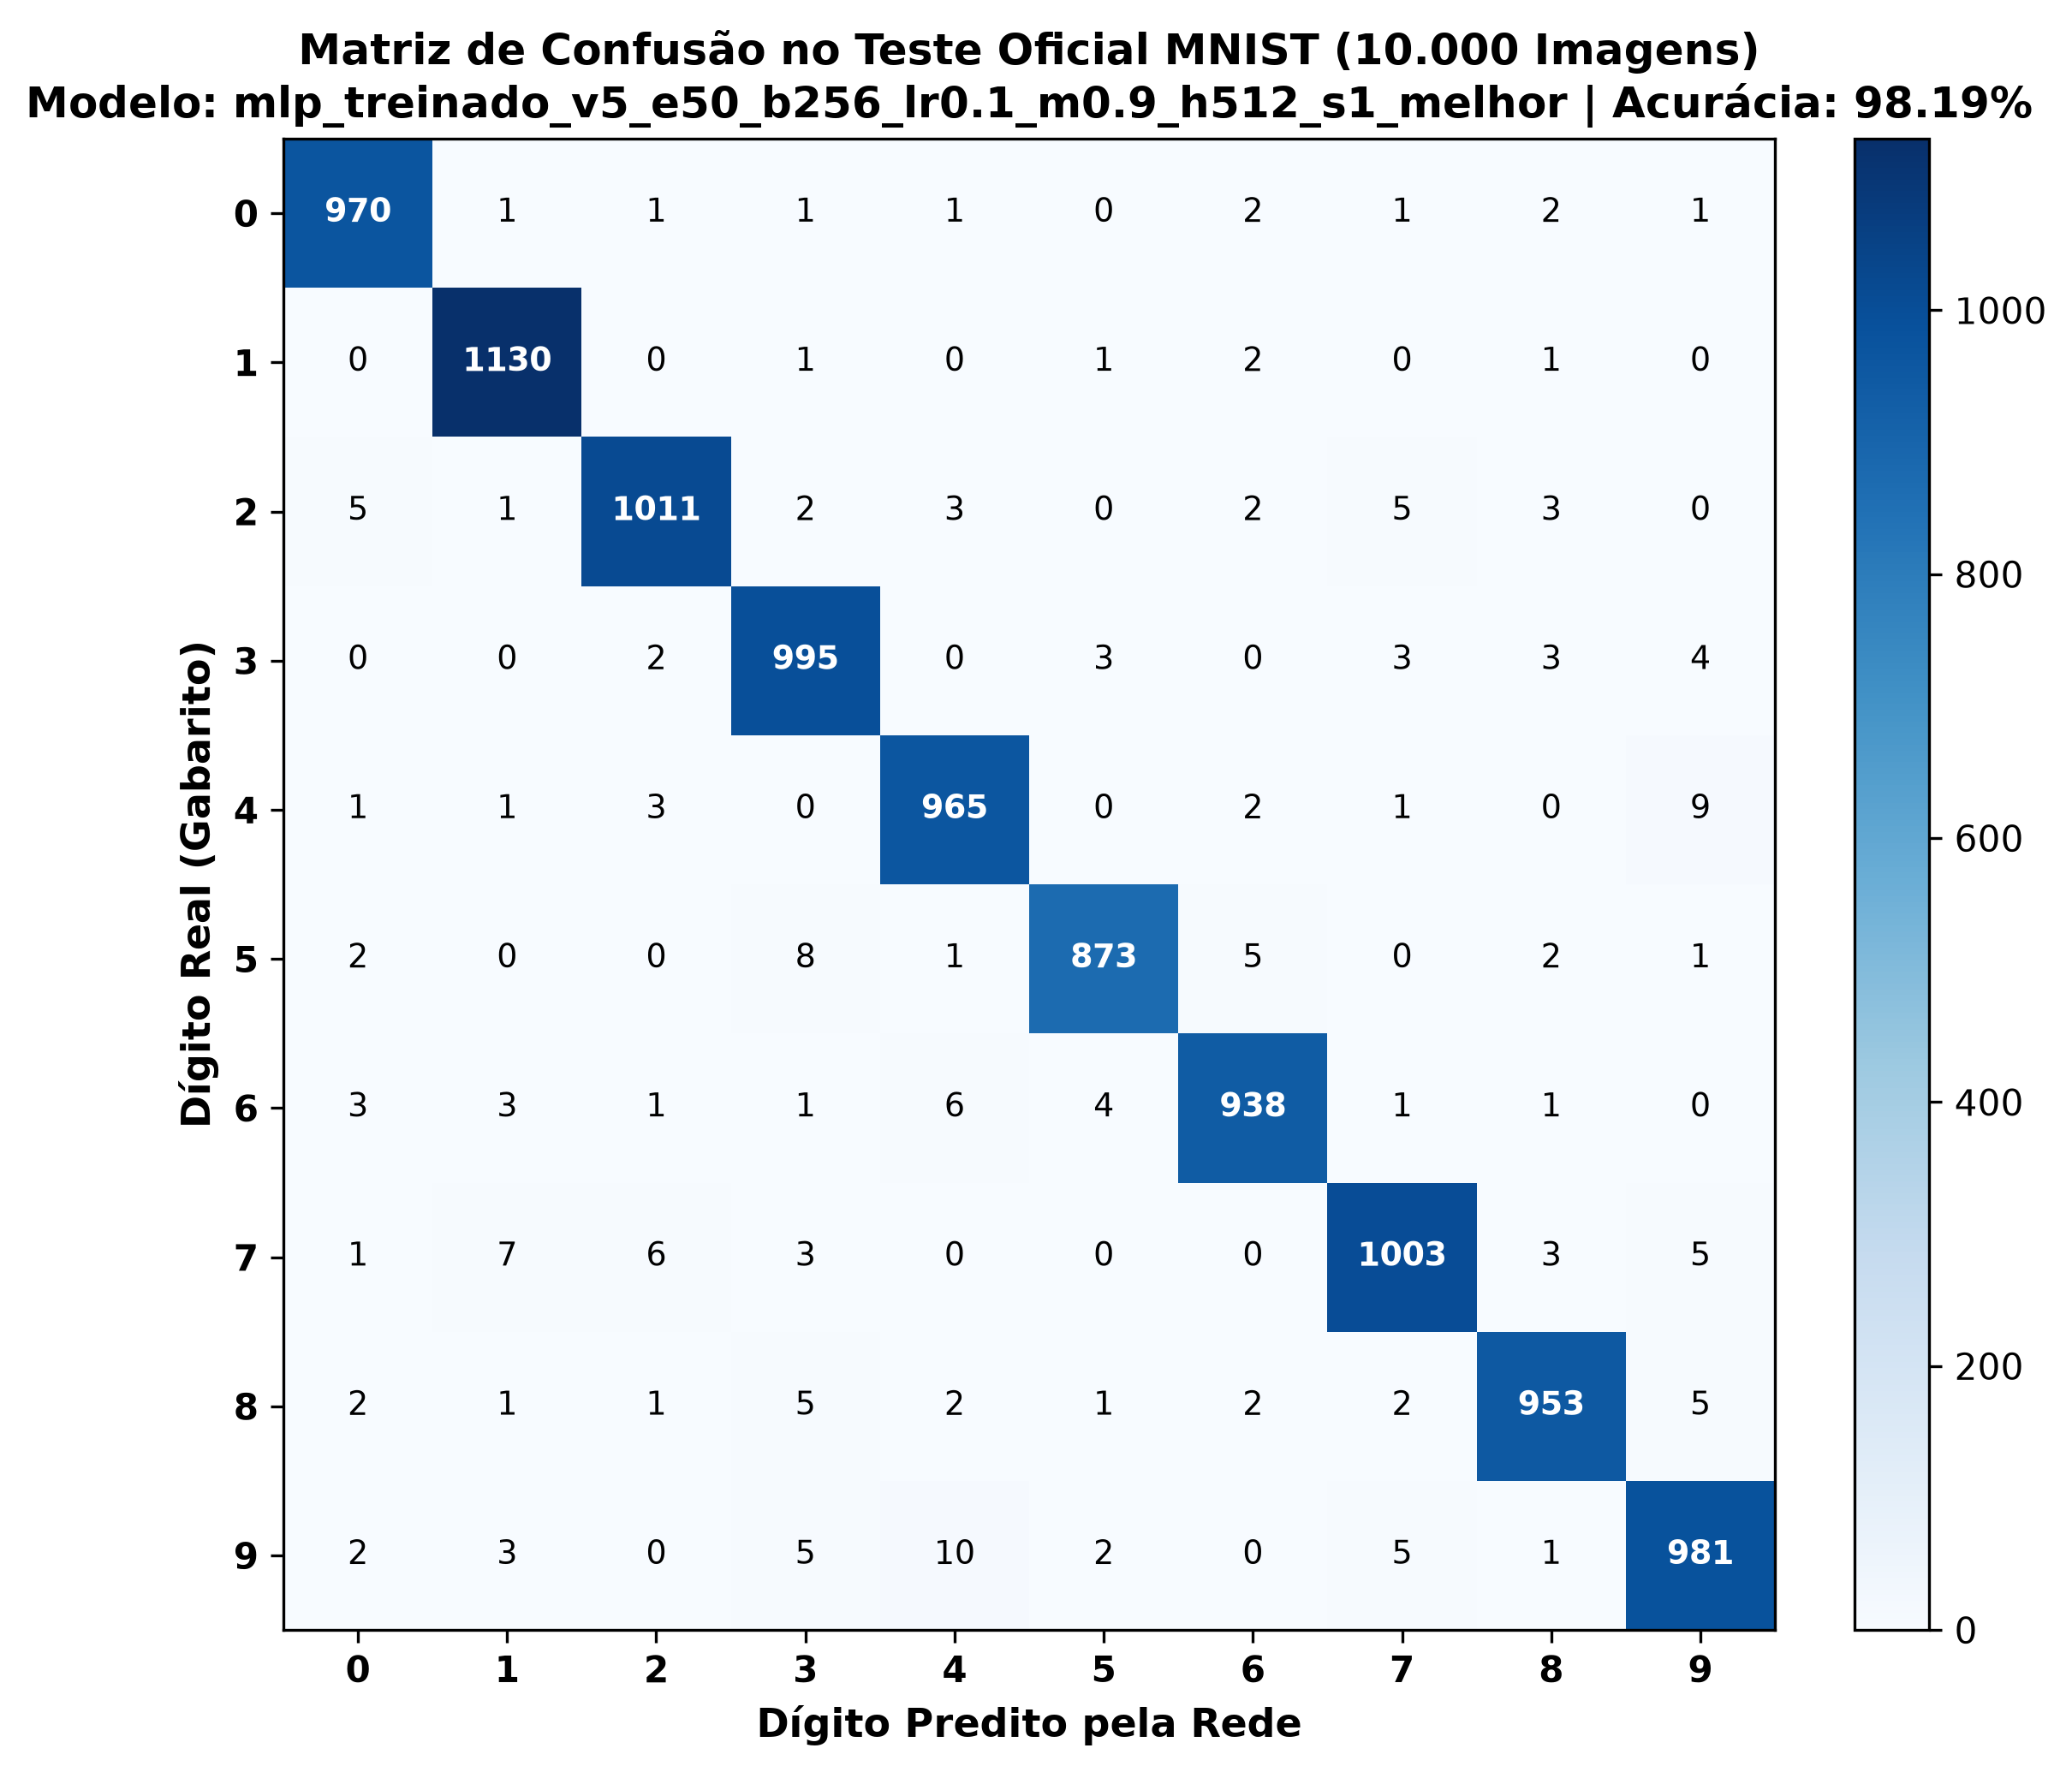
\includegraphics[width=0.62\columnwidth]{v5_e50_b256_lr0.1_m0.9_h512_s1/mlp_treinado_v5_e50_b256_lr0.1_m0.9_h512_s1_melhor_matriz_confusao.png}
\caption{Matriz de confusão do MLP campeão no teste ($98{,}19\%$).}
\label{fig:mlp_cm}
\end{figure}

Os erros do MLP não são aleatórios. Eles se acumulam em pares previsíveis: $9 \to 4$ ($10$ vezes), $4 \to 9$ ($9$ vezes), $5 \to 3$ ($8$ vezes), $7 \to 1$ ($7$ vezes), $6 \to 4$ ($6$ vezes) e $7 \to 2$ ($6$ vezes). Quando o traço sai inclinado ou corrido, o laço aberto do $9$ cai nos mesmos pixels absolutos da haste do $4$, o corte no meio do $7$ aciona regiões de $2$ ou $9$, e o bojo inferior compartilhado por $5$ e $3$ deixa tudo na conta de poucos pixels da quina superior esquerda.

\section{Redes Convolucionais}

\subsection{Sobre o Método}

As Redes Convolucionais mantêm a imagem em 2D usando três peças que trabalham juntas:
\begin{itemize}[nosep]
    \item \textbf{Convolução:} Filtros pequenos $K \times K$ ($5 \times 5$) correm sobre a grade calculando produtos escalares por região. Com $C_{\text{in}}$ canais de entrada, cada filtro vira um tensor $C_{\text{in}} \times K \times K$ que lê todos os canais juntos.
    \item \textbf{Compartilhamento de pesos:} Os mesmos $25$ pesos de um filtro varrem as $24 \times 24 = 576$ posições da primeira camada. Isso impõe equivariância à translação e corta a explosão de parâmetros.
    \item \textbf{Pooling:} O \texttt{MaxPool2d} ($2 \times 2$, passo $2$) guarda só a resposta máxima de cada bloco, abrindo mão da coordenada exata do pixel para ganhar invariância local a pequenos desvios e ampliar o campo receptivo na camada seguinte. Uma suspeita inicial era de que descartar $75\%$ das posições duas vezes seguidas apagaria traços finos e pioraria a troca entre $4$ e $9$. Na prática, os mapas seguintes provaram o oposto: guardar o pico local preserva a presença da borda e elimina a sensibilidade ao deslocamento milimétrico da caneta.
\end{itemize}

\subsection{Implementação (LeNet) e Gargalo Paramétrico}

Foi implementada a \texttt{LeNet}~\cite{lecun1998} em \texttt{models/cnn.py} para entrada $1 \times 28 \times 28$, ativações ReLU e saída em $10$ \textit{logits}:
{\small
\begin{equation*}
\begin{aligned}
(1,28,28) &\xrightarrow{\text{Conv1 }5\times 5} (6,24,24) \xrightarrow{\text{Pool}} (6,12,12) \\
&\xrightarrow{\text{Conv2 }5\times 5} (16,8,8) \xrightarrow{\text{Pool}} (16,4,4) \\
&\xrightarrow{\text{Flatten}} 256 \to 120 \to 84 \to 10
\end{aligned}
\end{equation*}
}

Como na linha \texttt{v5} do MLP, evitou-se encerrar o método \texttt{forward()} com \texttt{nn.Softmax}: como a \texttt{nn.CrossEntropyLoss} aplica \texttt{LogSoftmax} internamente, entregar probabilidades já normalizadas geraria um \textit{Softmax} duplo e achataria os gradientes. A arquitetura soma \textbf{$44.426$ parâmetros} ($89{,}1\%$ menos que o MLP). A contagem por bloco também desfez um erro inicial de estimativa para a \texttt{Conv2}: esperavam-se $16 \times (25 + 1) = 416$ pesos, tratando cada filtro como plano 2D. Como a \texttt{Conv1} entrega $6$ mapas de características, cada filtro da \texttt{Conv2} é um volume $5 \times 5 \times 6 + 1 = 151$ pesos, somando $2.416$ parâmetros ($5{,}44\%$). Somados aos $156$ da \texttt{Conv1} ($0{,}35\%$), as convoluções consomem apenas $2.572$ pesos ($5{,}79\%$). Os outros \textbf{$94{,}21\%$ ($41.854$)} ficam no classificador denso: \textbf{$30.840$ ($69{,}42\%$)} em \texttt{Linear(256, 120)}, $10.164$ ($22{,}88\%$) em \texttt{Linear(120, 84)} e $850$ ($1{,}91\%$) na saída \texttt{Linear(84, 10)}.

\subsection{Experimento e Confronto com o MLP}

O mesmo protocolo da bateria \texttt{v5} foi mantido na CPU para rodar a \texttt{cnn\_v1} ($4$ configurações de SGD com momento $0{,}9$ $\times$ $3$ sementes, $30$ épocas, Tabela~\ref{tab:cnn_val}). Na primeira tentativa, aplicou-se exatamente a configuração do MLP campeão ($\eta = 0{,}1$) por parecer a comparação mais justa entre arquiteturas. Enquanto as sementes $1$ e $2$ chegaram a $98{,}28\%$ e $98{,}33\%$, a semente $3$ colapsou já na época $1$. Travou por \textit{Dying ReLU} com $11{,}29\%$ de acurácia na validação (a proporção exata da classe majoritária $1$) e perda estagnada em $2{,}3027 \approx \ln 10$. A razão é física: como os gradientes de $576$ janelas espaciais se somam sobre os mesmos $25$ pesos do núcleo, passos largos com momento $0{,}9$ projetam as ativações para o lado negativo e zeram os gradientes da ReLU. Reduzir a taxa para $\eta = 0{,}02$ eliminou o colapso e unificou as três sementes ($98{,}73\%$, $98{,}69\%$ e $98{,}73\%$, desvio de $0{,}02\text{ p.p.}$). Na semente $1$, o mínimo de perda caiu na época $11$ ($0{,}0459$), embora a acurácia de validação ainda subisse até $99{,}07\%$ na época $30$ com perda de $0{,}0576$; seguiu-se o critério pré-definido de menor perda (Figura~\ref{fig:cnn_perda}).

\begin{table}[htbp]
\centering
\caption{Seleção da CNN LeNet na validação ($3$ sementes, $30$ épocas).}
\label{tab:cnn_val}
\resizebox{\columnwidth}{!}{%
\begin{tabular}{rrrrrr}
\toprule
Lote & $\eta$ & Acc Val (\%) & Perda Val & Ép. & Tempo (s) \\
\midrule
$256$ & $0{,}10$ & $69{,}30 \pm 50{,}24$ & $0{,}8147$ & $14{,}3$ & $97{,}0$ \\
$256$ & $0{,}05$ & $98{,}39 \pm 0{,}24$ & $0{,}0572$ & $8{,}0$ & $84{,}5$ \\
\textbf{$256$} & \textbf{$0{,}02$} & $\mathbf{98{,}72 \pm 0{,}02}$ & $\mathbf{0{,}0459}$ & $14{,}3$ & $86{,}1$ \\
$128$ & $0{,}05$ & $98{,}65 \pm 0{,}29$ & $0{,}0560$ & $17{,}7$ & $90{,}1$ \\
\bottomrule
\end{tabular}%
}
\end{table}

\begin{figure}[htbp]
\centering
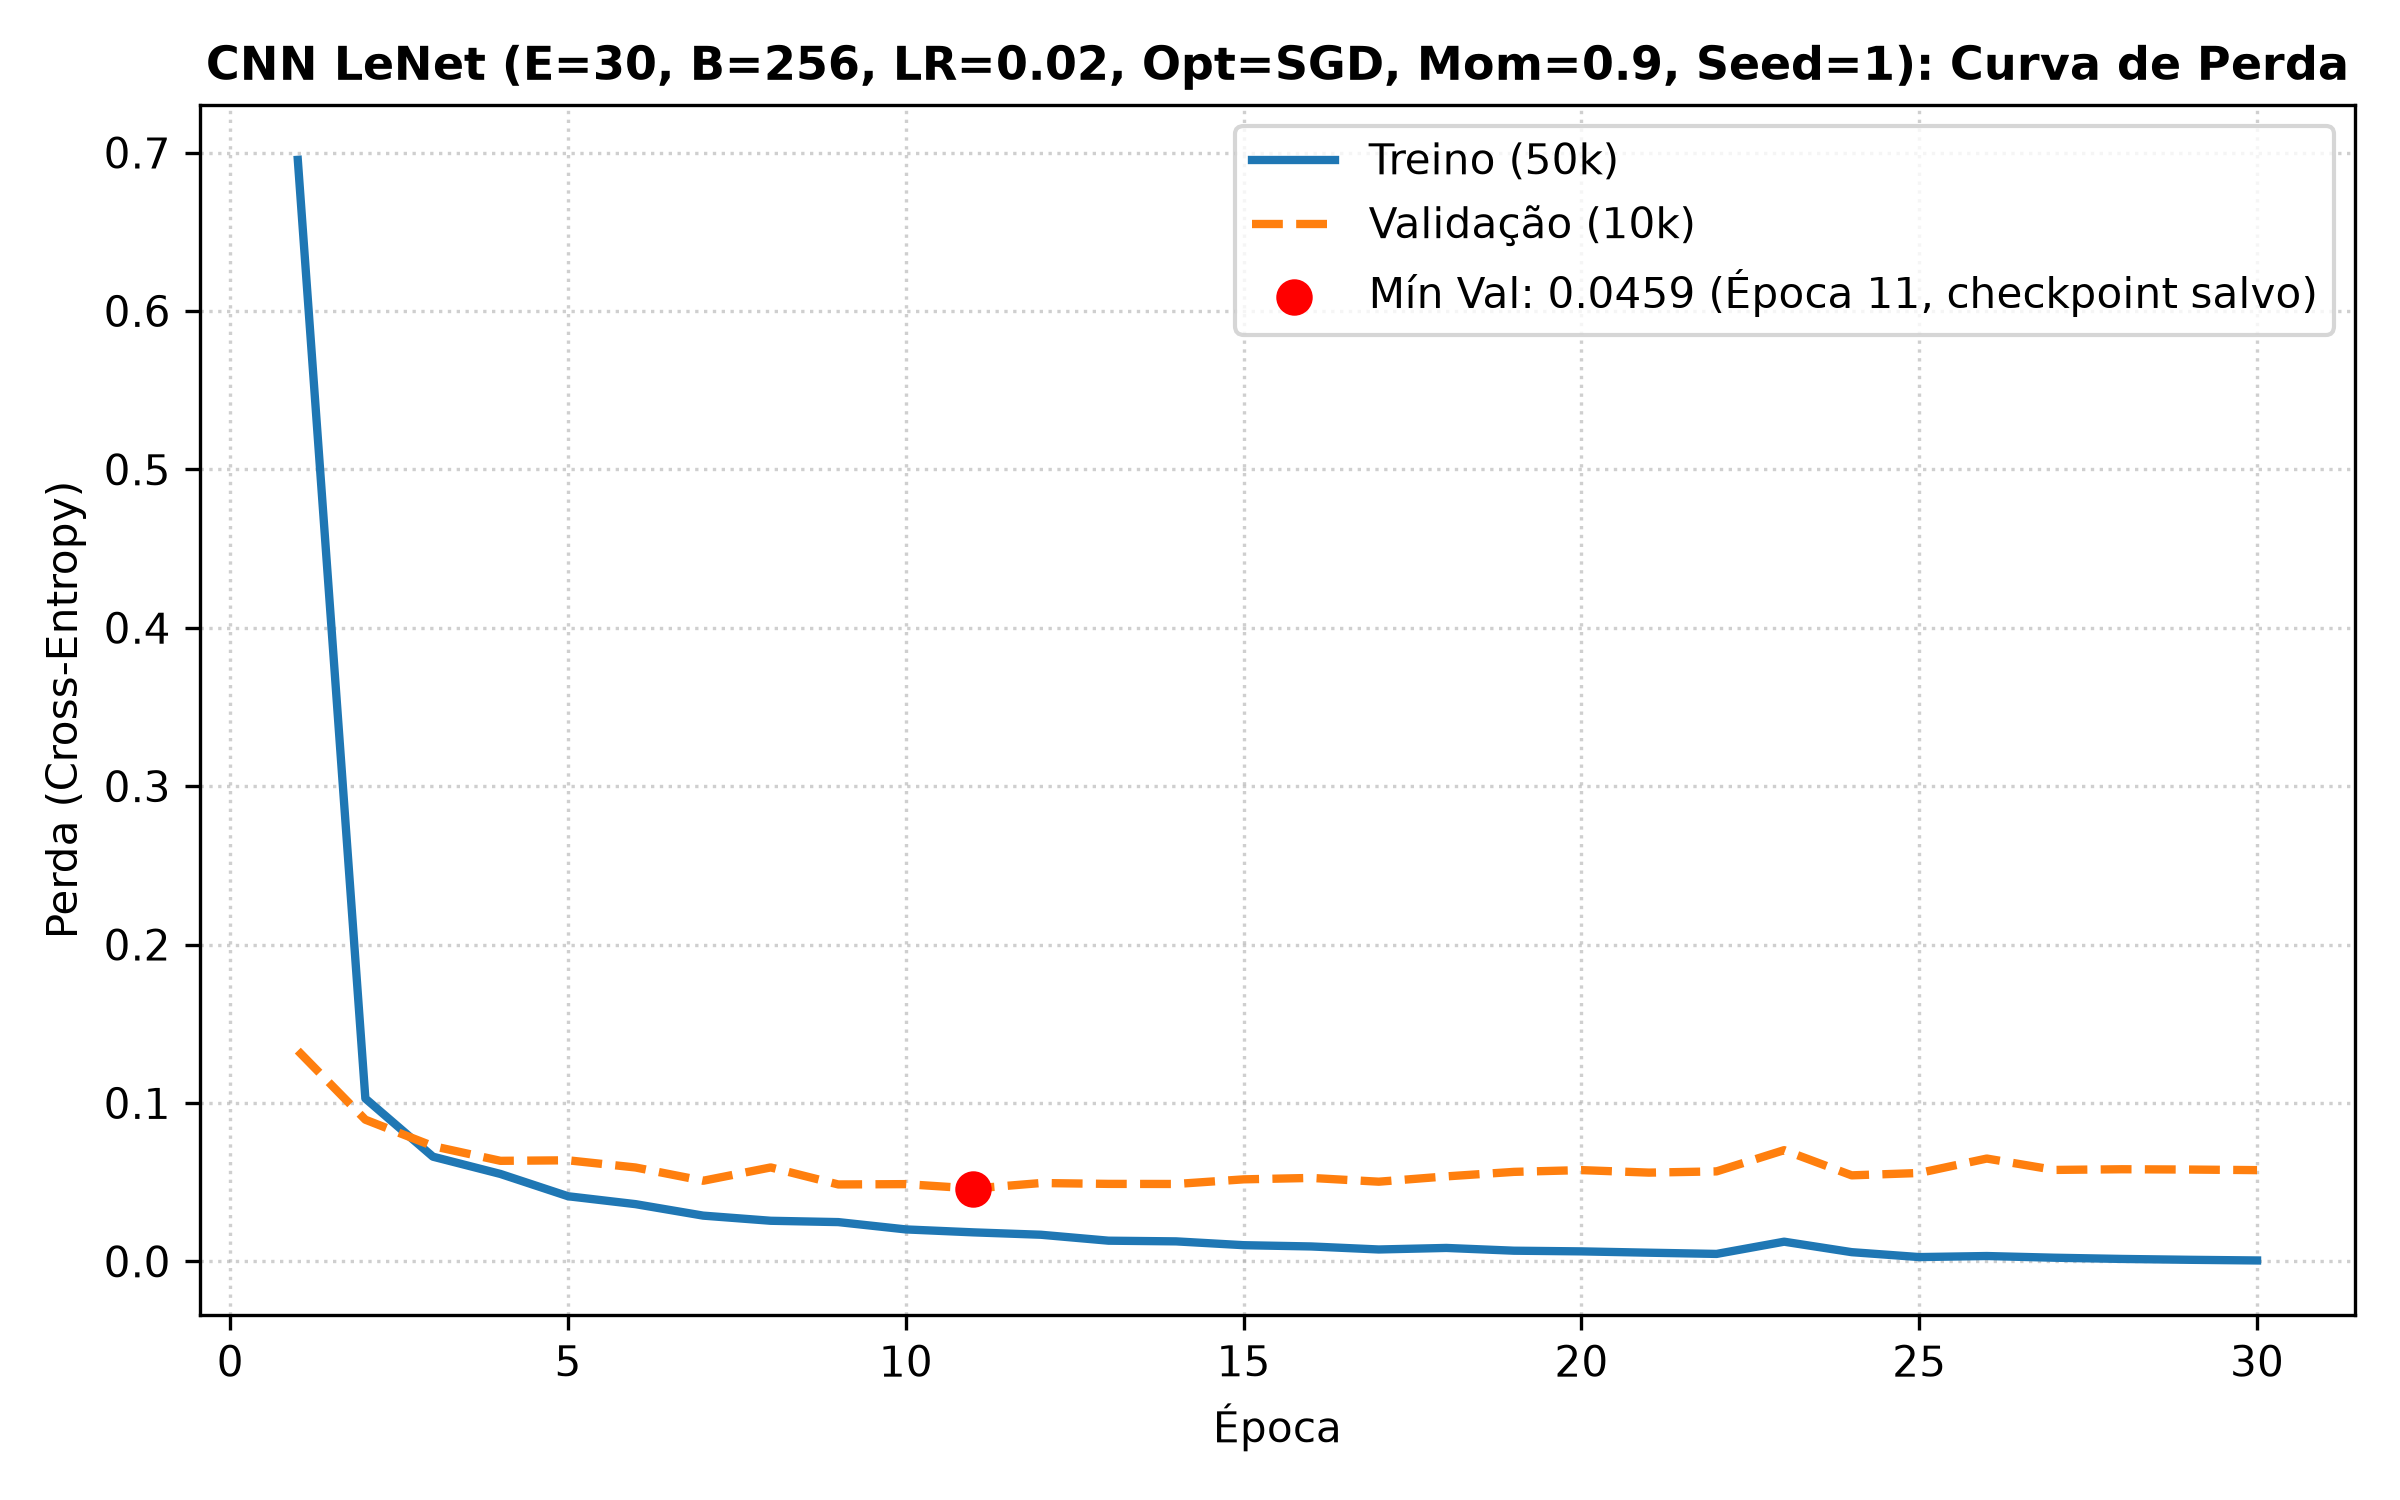
\includegraphics[width=0.74\columnwidth]{cnn_v1_e30_b256_lr0.02_m0.9_s1/cnn_treinado_v1_e30_b256_lr0.02_m0.9_s1_perda.png}
\caption{Curva de perda da CNN LeNet ($b=256, \eta=0{,}02, m=0{,}9$, mín.\ na época $11$).}
\label{fig:cnn_perda}
\end{figure}

No teste único oficial (\texttt{cnn\_v1\_testar.py}), a LeNet alcançou \textbf{$98{,}98\%$ de acurácia} ($102$ erros), perda de $0{,}03575$, precisão macro $98{,}99\%$, revocação macro $98{,}96\%$ e \textbf{F1 macro de $98{,}97\%$} (Figura~\ref{fig:cnn_cm}). A Tabela~\ref{tab:confronto} e a Figura~\ref{fig:confronto_ef} colocam os dois modelos lado a lado (\texttt{confronto\_mlp\_vs\_cnn.py}).

\begin{figure}[htbp]
\centering
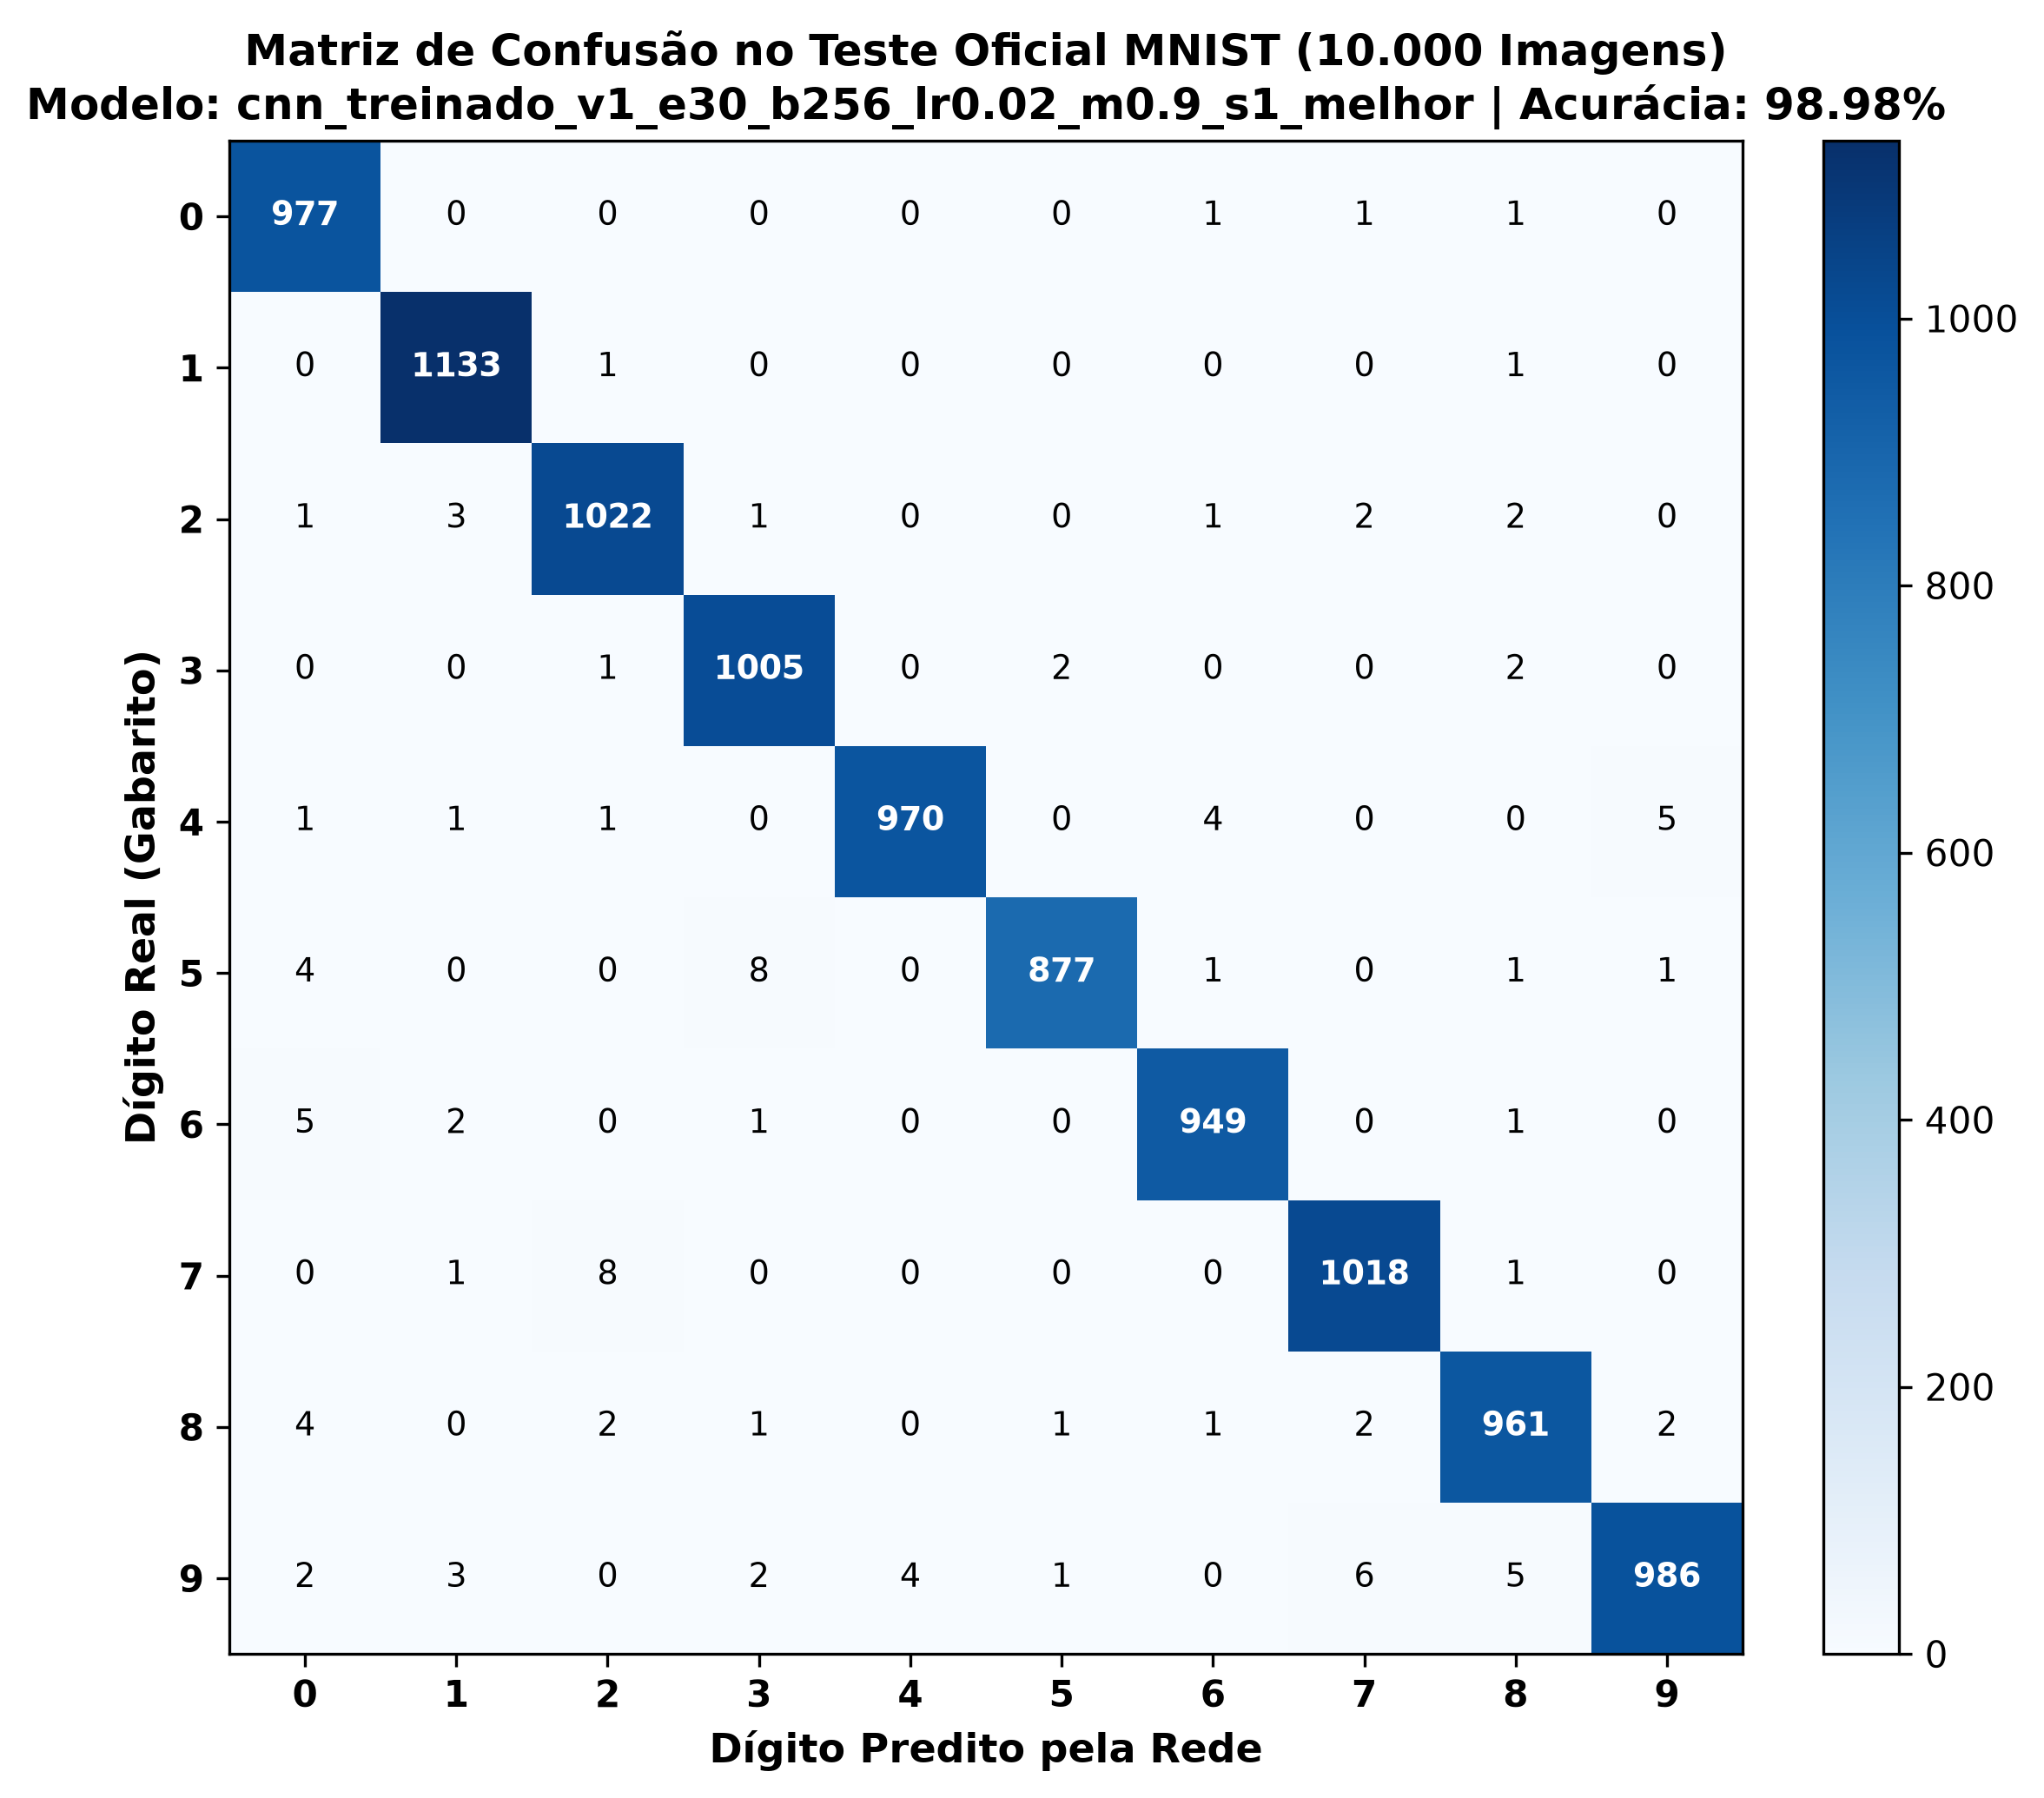
\includegraphics[width=0.60\columnwidth]{cnn_v1_e30_b256_lr0.02_m0.9_s1/cnn_treinado_v1_e30_b256_lr0.02_m0.9_s1_melhor_matriz_confusao.png}
\caption{Matriz de confusão da CNN LeNet no teste ($98{,}98\%$).}
\label{fig:cnn_cm}
\end{figure}

\begin{table}[htbp]
\centering
\caption{Confronto final no conjunto de teste oficial ($10.000$ amostras).}
\label{tab:confronto}
\resizebox{\columnwidth}{!}{%
\begin{tabular}{lrrr}
\toprule
Métrica & MLP Campeão & CNN LeNet & Variação \\
\midrule
Parâmetros treináveis & $407.050$ & $\mathbf{44.426}$ & $-89{,}1\%$ \\
Acurácia no teste (\%) & $98{,}19\%$ & $\mathbf{98{,}98\%}$ & $+0{,}79\text{ p.p.}$ \\
Erros no teste ($/10\text{k}$) & $181$ & $\mathbf{102}$ & $-43{,}6\%$ \\
Macro-F1 (\%) & $98{,}18\%$ & $\mathbf{98{,}97\%}$ & $+0{,}79\text{ p.p.}$ \\
Perda média no teste & $0{,}06039$ & $\mathbf{0{,}03575}$ & $-40{,}8\%$ \\
Tempo total de treino (CPU) & $\mathbf{53{,}03\text{ s}}$ ($50$ ép.) & $85{,}84\text{ s}$ ($30$ ép.) & $+61{,}9\%$ \\
Tempo por época (CPU) & $\approx \mathbf{1{,}06\text{ s}}$ & $2{,}86\text{ s}$ & $2{,}70\times$ \\
\bottomrule
\end{tabular}%
}
\end{table}

\begin{figure}[htbp]
\centering
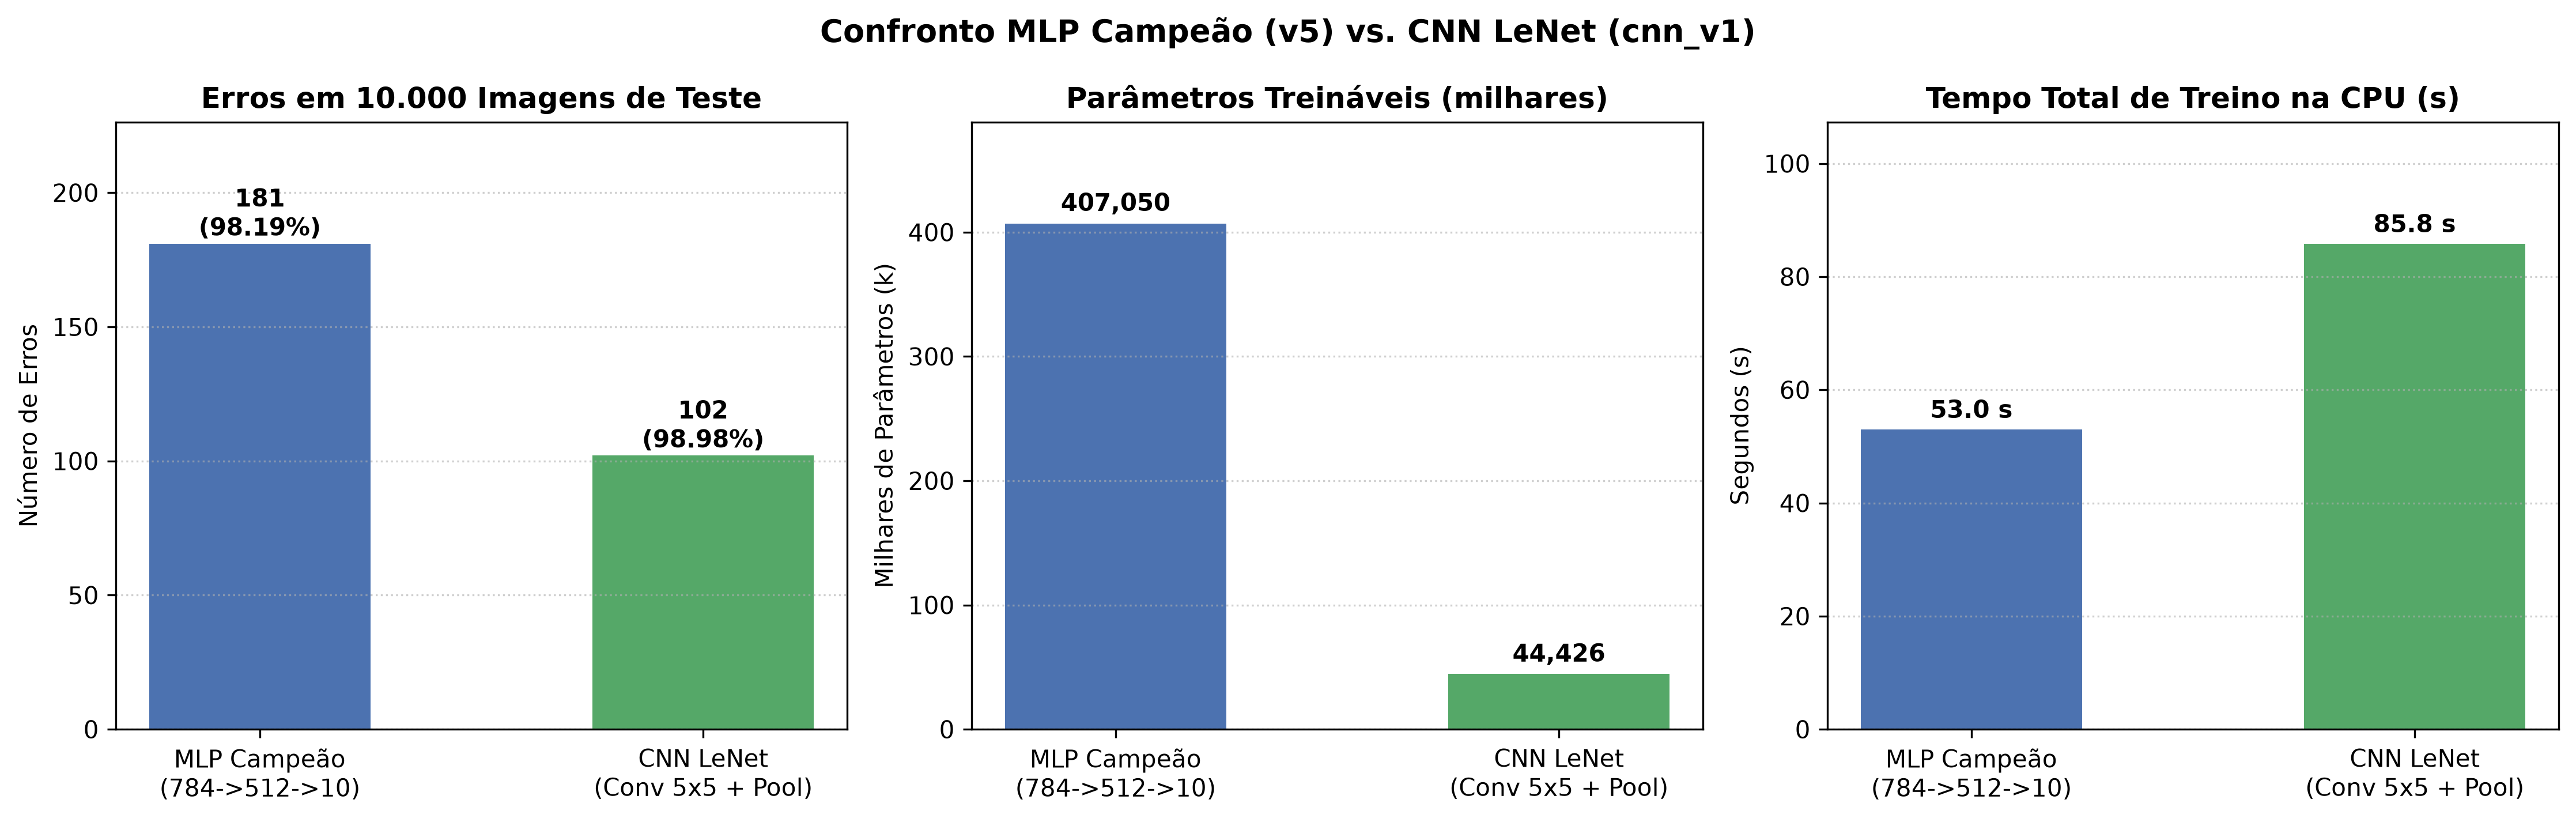
\includegraphics[width=0.92\columnwidth]{confronto_mlp_vs_cnn/confronto_eficiencia.png}
\caption{Confronto MLP Campeão vs.\ CNN LeNet: erros, parâmetros e tempo na CPU.}
\label{fig:confronto_ef}
\end{figure}

A troca é direta: são economizados $89{,}1\%$ dos pesos e os erros caem $43{,}6\%$, ao custo de épocas $2{,}70\times$ mais lentas na CPU. Poucos pesos não significam pouca conta. Na matriz densa, cada peso entra em uma multiplicação por imagem; na convolução, cada peso varre centenas de janelas espaciais. O mesmo padrão reaparece na inferência das $10.000$ amostras de teste, onde a LeNet levou $0{,}241\text{ s}$ contra $0{,}1163\text{ s}$ do MLP (\texttt{confronto\_mlp\_vs\_cnn.json}).

\medskip
\noindent\textbf{Análise Morfológica das Confusões.} Pareando as predições nos $10.000$ dígitos de teste, os dois modelos acertaram juntos $9.780$ vezes, a \textbf{CNN corrigiu o MLP em $118$ dígitos}, perdeu para ele em $39$ e ambos erraram $63$. Comparando as matrizes (Figuras~\ref{fig:mlp_cm} e~\ref{fig:cnn_cm}) com os exemplos reais da Figura~\ref{fig:galeria}, os filtros espaciais desarmaram justamente os erros geométricos do MLP: $9 \to 4$ caiu de $10$ para $4$ ($-60\%$), $4 \to 9$ de $9$ para $5$ ($-44\%$), $7 \to 1$ de $7$ para $1$ ($-86\%$), $7 \to 9$ de $5$ para $0$ ($-100\%$), $6 \to 4$ de $6$ para $0$ ($-100\%$) e $8 \to 3$ de $5$ para $1$ ($-80\%$). Dígitos $7$ cortados no meio, $6$ fechados e $2$ ou $3$ deslocados da moldura voltaram a fazer sentido para a rede. Em sentido oposto, nos $39$ casos em que o MLP acertou e a CNN falhou, destaca-se o aumento de $7 \to 2$ (de $6$ para $8$ ocorrências), indicando que o \textit{pooling} $2 \times 2$ ocasionalmente suaviza um traço curto na base de dígitos inclinados. Já o empate de $8$ erros em $5 \to 3$ e o núcleo de $63$ falhas conjuntas mostram que, quando a quina superior do $5$ quase some no traço manuscrito, falta sinal visual para qualquer uma das duas arquiteturas.

\begin{figure}[htbp]
\centering
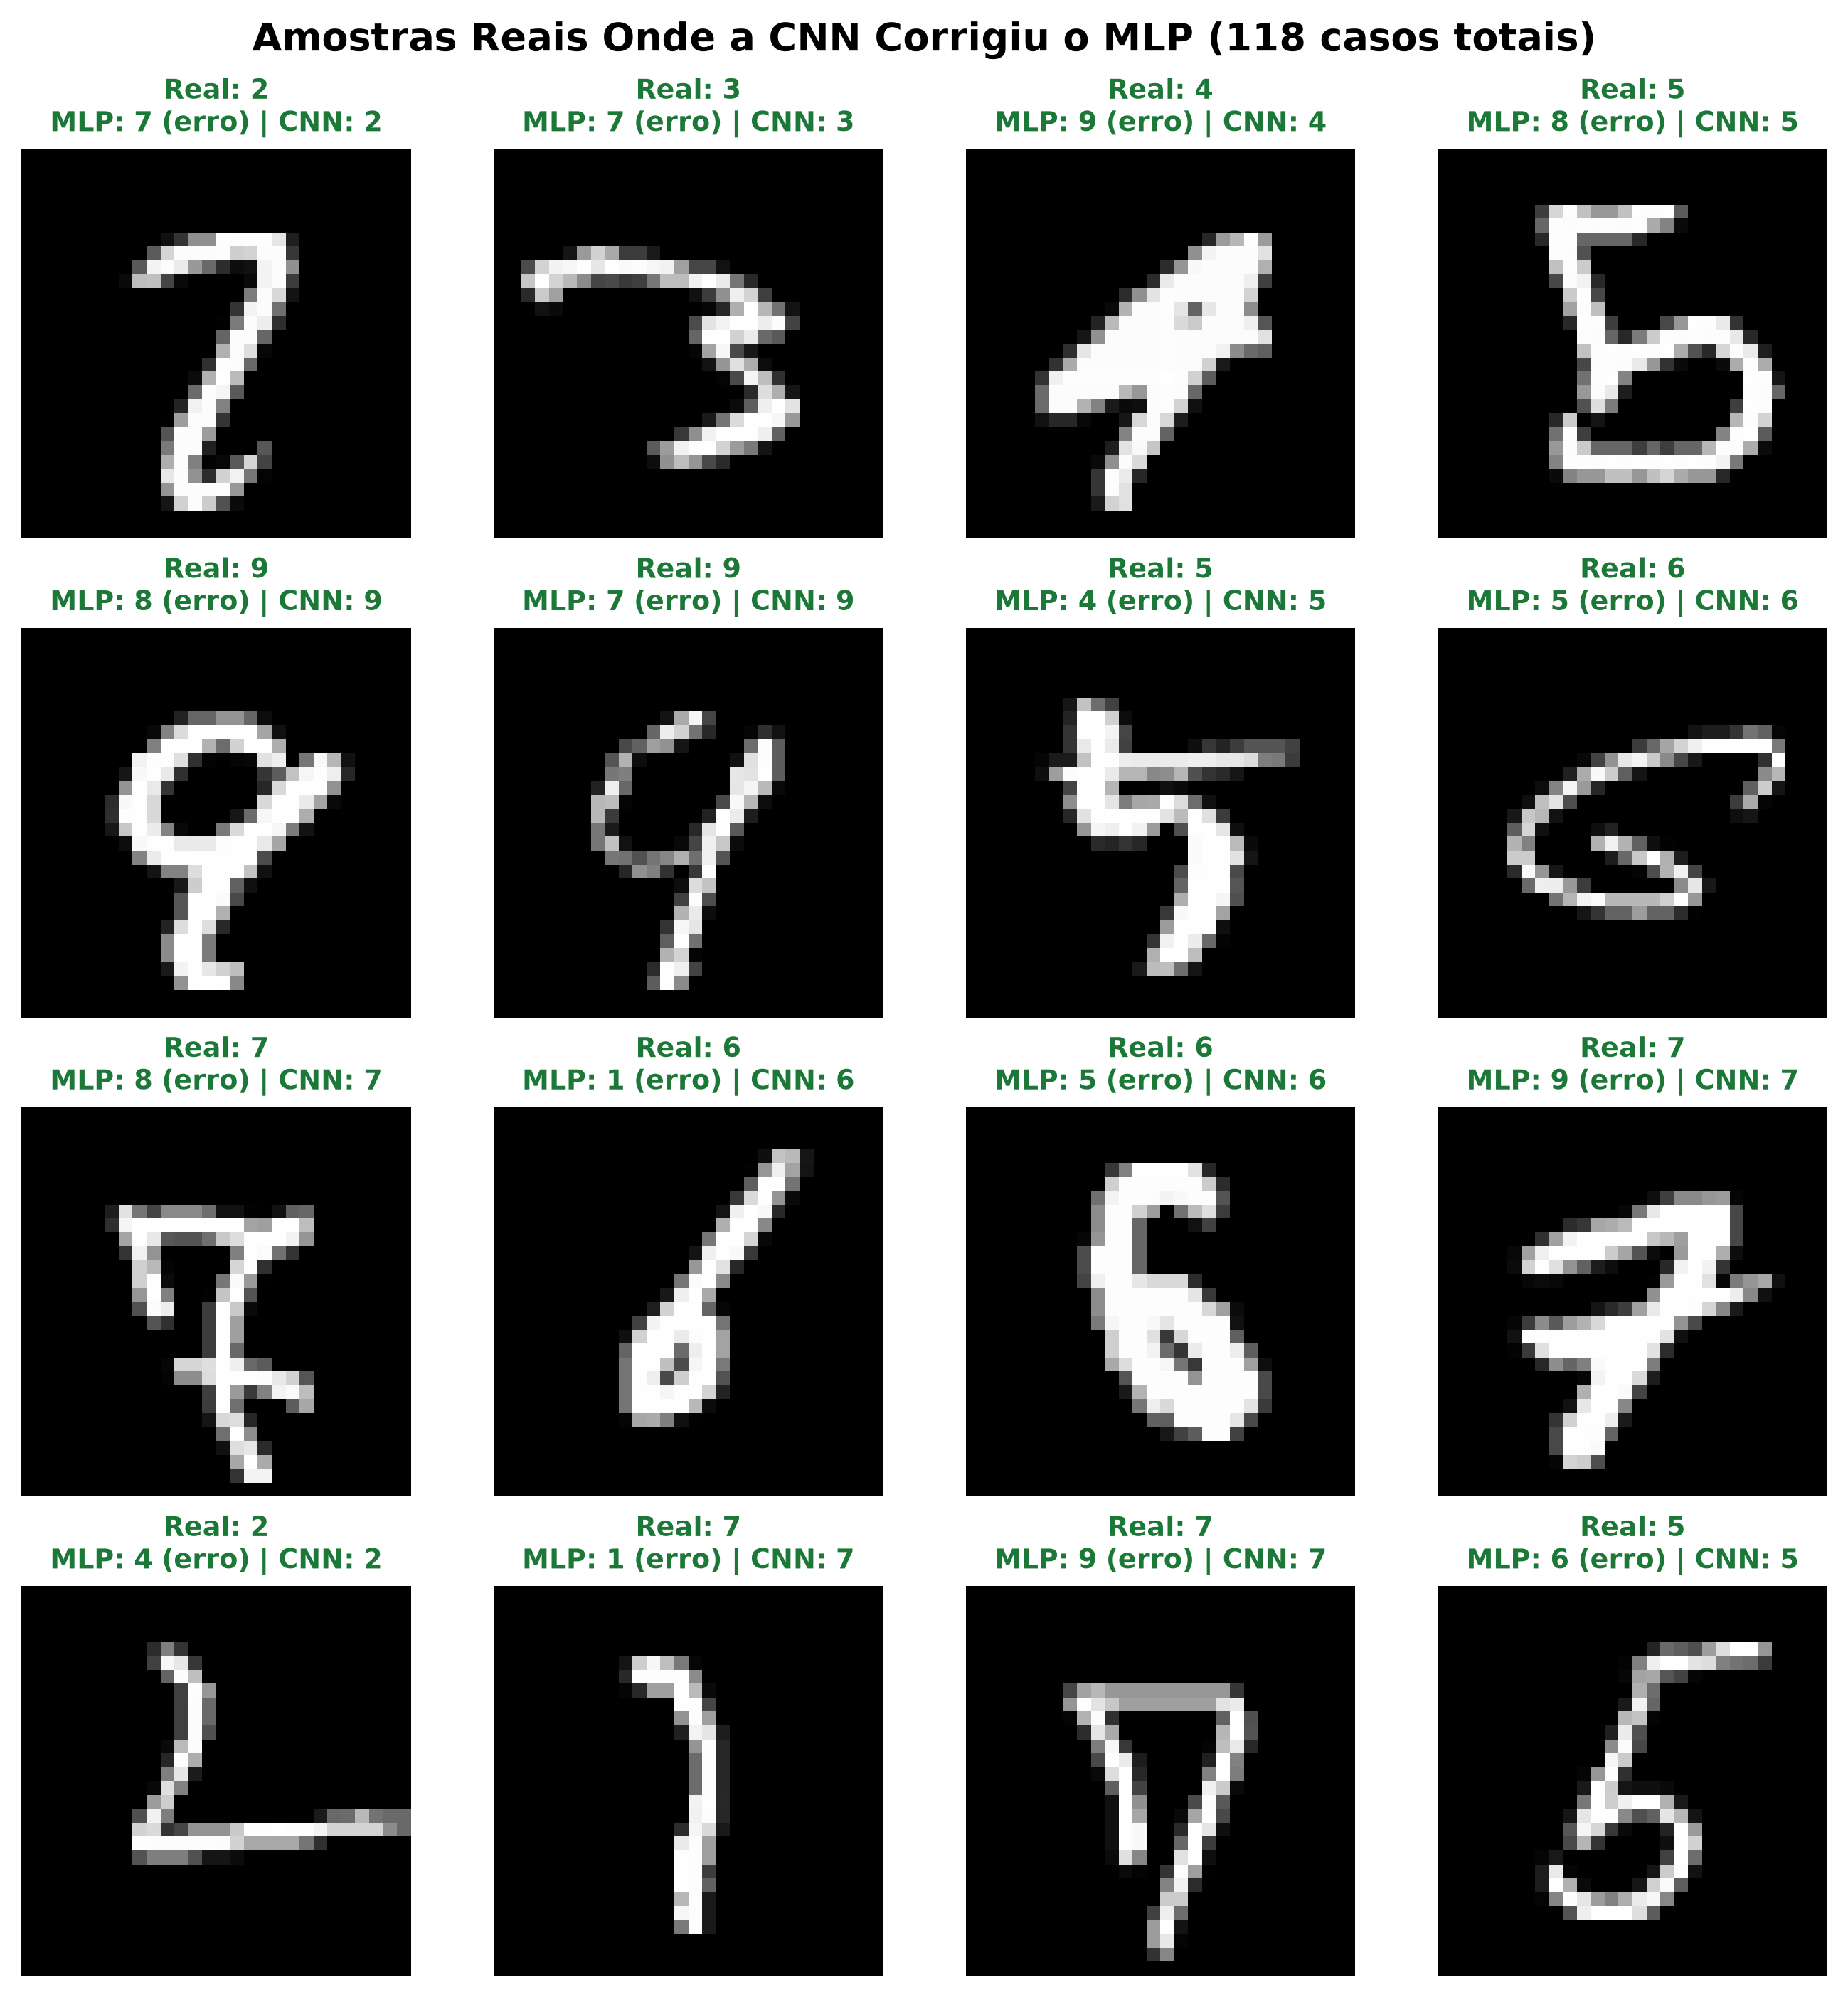
\includegraphics[width=0.52\columnwidth]{confronto_mlp_vs_cnn/confronto_cnn_corrige_mlp.png}
\caption{Amostras de teste em que o MLP falhou e a CNN LeNet acertou.}
\label{fig:galeria}
\end{figure}

\section{Considerações Finais}

Preservar a grade 2D decidiu o experimento. A LeNet reduziu os erros de $181$ para $102$ no teste ($98{,}98\%$ de acurácia e $98{,}97\%$ de F1 macro) carregando $44.426$ parâmetros contra $407.050$ do MLP, ao custo de épocas $2{,}70\times$ mais pesadas na CPU. Pelo caminho, selecionar tudo na validação antes de abrir o conjunto de teste corrigiu impressões que pareciam razoáveis no papel: revelou que o critério de perda muda a leitura sobre profundidade no MLP, desfez a hipótese de que o \textit{pooling} apagaria distinções finas e mostrou que importar $\eta = 0{,}1$ direto para a CNN dispara \textit{Dying ReLU} na época $1$. Como evolução natural, o diagnóstico de que $94{,}21\%$ dos pesos da LeNet ainda ficam concentrados no classificador denso aponta para a substituição de camadas lineares largas por \textit{Global Average Pooling} em arquiteturas maiores.

\begin{thebibliography}{00}
\footnotesize
\setlength{\itemsep}{0pt}
\setlength{\parskip}{0pt}
\bibitem{russell2020}
RUSSELL, S.; NORVIG, P. \textbf{Artificial Intelligence: A Modern Approach}. 4. ed. Pearson, 2020. Cap. 22: Deep Learning.

\bibitem{smola2023}
SMOLA, A. et al. \textbf{Dive into Deep Learning}. Cambridge University Press, 2023. Caps. 4, 5 e 7.

\bibitem{lecun1998}
LECUN, Y. et al. Gradient-Based Learning Applied to Document Recognition. \textbf{Proceedings of the IEEE}, v. 86, n. 11, p. 2278--2324, 1998.

\bibitem{paszke2019}
PASZKE, A. et al. PyTorch: An Imperative Style, High-Performance Deep Learning Library. \textbf{NeurIPS 32}, p. 8024--8035, 2019.
\end{thebibliography}

\end{document}
